% ================================================================================
% Pastikan isi semua data pada file "properti_dokumen.tex" di folder "konfigurasi"
% ================================================================================


% Memanggil Package MathFmipaUnmul yang telah dibuat
\documentclass{konfigurasi/MathFmipaUnmul}

% Memasukkan properti data dari file lain yang telah dikonfigurasi
% ========================================================================
%                 ------ INPUT DATA PROPERTI DOKUMEN  ------
% ========================================================================

% Masukkan tahap naskah, pilih salah satu : {sempro/semhas/pendadaran/pengesahan}
% Pastikan ditulis dengan huruf kecil
\var{\tahap}{semhas}

% Variabel tipe naskah
% Nilai akan menyesuaikan dengan input \tahap di atas secara otomatis
\ifthenelse{\equal{\tahap}{sempro}}{
    \var{\tipe}{Proposal Skripsi}
    \Var{\Tipe}{Proposal Skripsi}
}{
    \ifthenelse{\equal{\tahap}{semhas}}{
        \var{\tipe}{Draf Skripsi}
        \Var{\Tipe}{Draf Skripsi}
    }{
        \ifthenelse{\equal{\tahap}{pendadaran}}{
            \var{\tipe}{Draf Skripsi}
            \Var{\Tipe}{Draf Skripsi}
        }{
            % Todo for "pengesahan"
            \var{\tipe}{Skripsi}
            \Var{\Tipe}{Skripsi}
        }
    }
}

% Masukkan judul dalam bahasa Indonesia di sini
\Var{\Judul}{Optimalisasi Pemilihan Urutan Syuting \textit{Scene} Film \\ Menggunakan Algoritma \textit{Particle Swarm Optimization}}
\var{\subjudul}{Studi Kasus: Film "Ketika Adzan Sudah Tidak Lagi Berkumandang"}
\var{\judul}{Optimalisasi Pemilihan Urutan Syuting \textit{Scene} Film Menggunakan Algoritma \textit{Particle Swarm Optimization} (\subjudul)}

% Masukkan data diri mahasiswa di sini
\var{\mahasiswa}{Langgeng Prassadewo Sukma Adi Winoto Basla}
\var{\nim}{1807065014}
\var{\email}{langgengprassadewo@gmail.com}
\var{\kontak}{082238691473}

% Masukkan hari dan tanggal ujian
\var{\hari}{Jumat}
\var{\tanggalujian}{07 Maret 2025}

% Masukkan tanggal penelitian
\var{\tanggalpenelitian}{07 Maret 2025}

% Variabel data pembimbing naskah ini
\var{\pembimbinga}{Wasono, S.Si., M.Si.}
\var{\nipa}{NIP. 19810712 202321 1 011}
\var{\pembimbingb}{Fidia Deny Tisna Amijaya, S.Si., M.Si.}
\var{\nipb}{NIP. 19880201 201504 1 033}

% Variabel data penguji naskah ini
\var{\pengujia}{Dr. Syaripuddin, S.Si., M.Si.}
\var{\nippa}{19740112 200012 1 002}
\var{\pengujib}{Andri Azmul Fauzi, S.Si., M.Si.}
\var{\nippb}{19920608 202321 1 023}


% Varianel data pejabat jurusan dan prodi
\var{\kajur}{Dr. Syaripuddin, M.Si.}
\var{\jabatankajur}{Ketua \jurusan, \fakultas, \institut, \kota}
\var{\korprodi}{Qonita Qurrota A\'yun, S.Si., M.Sc.}
\var{\jabatankorprodi}{Koordinator \prodi, \fakultas, \institut, \kota}


% Variabel data perguruan tinggi dan fakultas
\var{\dekan}{Dr. Dra. Hj. Ratna Kusuma, M.Si.}
\var{\nipdekan}{19630416 198903 2 002}
\var{\kota}{Samarinda}
\Var{\Kota}{Samarinda}
\var{\tahun}{2025}
\var{\tingkat}{Sarjana}
\var{\institut}{Universitas Mulawarman}
\Var{\Institut}{UNIVERSITAS MULAWARMAN}
\var{\fakultas}{Fakultas Matematika dan Ilmu Pengetahuan Alam}
\Var{\Fakultas}{FAKULTAS MATEMATIKA DAN ILMU PENGETAHUAN ALAM}
\var{\jurusan}{Jurusan Matematika}
\Var{\Jurusan}{JURUSAN MATEMATIKA}
\var{\prodi}{Program Studi S1 Matematika}
\Var{\Prodi}{PROGRAM STUDI S1 MATEMATIKA}
\var{\strata}{Sarjana Matematika}
\Var{\Strata}{SARJANA MATEMATIKA}
\var{\prasyarat}{Diajukan Sebagai Persyaratan Memperoleh Gelar \strata~pada \prodi,~\jurusan,~\institut}

\hyphenation{
    pro-per-ti
    ber-bo-bot
    mung-kin
    ber-a-rah
    par-ti-cle
    me-ne-ri-ma
    ber-in-ter-ak-si
    be-be-ra-pa
    ber-pa-sa-ngan
    cen-ter
    da-ri
    de-ngan
    di-kontinu-asi
    di-se-ki-tar
    ekuili-brium
    e-ner-gi
    fung-si
    fe-no-me-na
    ins-ti-tut
    tek-no-lo-gi
    ban-dung
    ja-co-bian
    ke-stabilan
    kon-ti-nuasi
    meng-awet-kan
    me-nyatakan
    para-meter
    pe-ra-ta-an
    peri-la-ku
    peri-la-ku-nya
    pe-riodik
    ruang
    sa-ling
    se-dang-kan
    suatu
    sta-bil
    ter-di-fe-ren-sial-kan
    tri-vial
    o-si-la-tor
    ke-tak-linearan-nya
    meng-gu-na-kan
    de-fi-ni-si
    si-mu-la-tor
    o-pe-ra-ting
    per-ta-mi-na
    de-ve-lop-ment
    meng-iden-ti-fi-ka-si
    bi-la-ngan
    me-nya-ta-kan
    mo-di-fi-ka-si
    a-na-li-sis
    ke-mung-ki-nan
    mo-del-ling
    geo-met-ri-ka
    o-ri-gi-nal
    de-ngan
    ja-nuari
}
\addbibresource{daftar_pustaka/daftar_pustaka.bib}

% ========================================================================
%                            KERANGKA DOKUMEN
% ========================================================================
\begin{document}

% -------------------------- Bagian Awal ---------------------------------

% => Halaman Sampul Luar
% Pengaturan posisi nomor halaman untuk sampul luar
\thispagestyle{empty}

% Pengaturan margin untuk halaman sampul luar
\newgeometry{left = 3cm, top = 3cm, right = 3cm, bottom = 3cm}

\frenchspacing
\begin{center}
    % Judul Tulisan
    \tb{\Judul \\ (\subjudul)}
    \vfill

    % Tipe Naskah
    \tb{\large\Tipe}
    \vfill

    % Logo Universitas Mulawarman
    
\includegraphics[width = 3.45cm]{gambar/logo.png}
    \vfill

    % Identitas Mahasiswa Penulis
    \tb{\mahasiswa \\ NIM. \nim}
    \vfill

    % Informasi Institut
    \tb{\Prodi \\ \Jurusan \\ \Fakultas \\ \Institut \\ \Kota \\ \tahun}
\end{center}

\pagebreak

% Mengembalikan margin seperti sebelumnya
\restoregeometry

% Pemberian nomor halaman i sesi ini dimulai dari halaman ini
\pagenumbering{roman}
\setcounter{page}{1}

% => Halaman Sampul Dalam
% Menambahkan "Halaman Judul" ke dalam daftar isi
\addChapter{HALAMAN JUDUL}

% Pengaturan format nomor halaman untuk Halaman sampul dalam sampai sebelum Bab 1
\pagestyle{fancy}
\lhead{}
\chead{}
\rhead{}
\lfoot{}
\cfoot{\thepage}
\rfoot{}

% ======================================================================

\frenchspacing
\begin{center}
  \tb{\Judul \\ (\subjudul)}
  \vfill

  \tb{\large\Tipe}
  \vfill

  \tb{Diajukan kepada}

  \tb{\jurusan~\fakultas}

  \tb{\institut~ untuk memenuhi sebagai persyaratan \\ memperoleh gelar \strata}
  \vfill

  \tb{Oleh: \\ \mahasiswa \\ NIM. \nim}
  \vfill

  \tb{\Prodi \\ \Jurusan \\ \Fakultas \\ \Institut \\ \Kota \\ \tahun}
\end{center}

\pagebreak


% Pengaturan format otomatis untuk susunan lembar pernyataan, pengesahan, dll mengikuti value \tahap
\ifthenelse{\equal{\tahap}{semhas}}{
  % => Lembar pengesahan
  % 
\addChapter{LEMBAR PENGESAHAN}

% =====================================================================
\frenchspacing
\begin{center}
    \textbf{HALAMAN PENGESAHAN}
\end{center}
\vspace{3mm}

  % => Abstrak
  \input{badan_skripsi/00_Abstrak}

  % => Abstract
  \input{badan_skripsi/00_Abstract}
}{
  \ifthenelse{\equal{\tahap}{pendadaran}}{
    % => Lembar pengesahan
    % 
\addChapter{LEMBAR PENGESAHAN}

% =====================================================================
\frenchspacing
\begin{center}
    \textbf{HALAMAN PENGESAHAN}
\end{center}
\vspace{3mm}

    % => Abstrak
    \input{badan_skripsi/00_Abstrak}

    % => Abstract
    \input{badan_skripsi/00_Abstract}
  }{
    \ifthenelse{\equal{\tahap}{pengesahan}}{
      % => Lembar pernyataan
      % Menambahkan "Pernyataan keaslian skripsi" ke dalam daftar isi
\addChapter{PERNYATAAN KEASLIAN SKRIPSI}

% Mengatur jarak spasi baris
\setstretch{1.4}

% =====================================================================
\frenchspacing
\begin{center}
    \tb{PERNYATAAN KEASLIAN SKRIPSI}
\end{center}
\vspace{3mm}

{\singlespacing % mengatur spasi menjadi single untuk semua di dalam {}
    Dengan ini saya menyatakan dengan sesungguhnya bahwa \tipe~ yang berjudul
    "\judul" tidak terdapat karya yang pernah diajukan untuk memperoleh gelar
    \strata~ di suatu perguruan tinggi mana pun.
    Sepanjang pengetahuan saya, tidak terdapat karya atau pendapat yang pernah
    ditulis atau diterbitkan oleh orang lain, kecuali yang secara tertulis
    diacu dalam naskah ini dan disebutkan dalam daftar pustaka.

    Demikian pernyataan ini dibuat dengan sebenar-benarnya.
    Saya sanggup menerima konsekuensi akademik di kemudian hari apabila pernyataan
    yang dibuat ini tidak benar
}

{\onehalfspacing % mengatur spasi menjadi onehalfspacing untuk semua di dalam {}
    \vspace{8mm}
    \begin{flushright}
        \begin{tabular}{l}
            \kota, \tanggalujian \\
            \\
            \hspace{-6cm}\framebox[1.1\width]{\ti{\footnotesize Materai 10.000}}
            \\
            \\
            \textbf{\mahasiswa}
        \end{tabular}
    \end{flushright}
}

\pagebreak

      % => Lembar pengesahan
      % 
\addChapter{LEMBAR PENGESAHAN}

% =====================================================================
\frenchspacing
\begin{center}
    \textbf{HALAMAN PENGESAHAN}
\end{center}
\vspace{3mm}

      % => Lembar Kelulusan
      \input{perangkat_skripsi/05_Hal_Kelulusan}

      % => Lembar publikasi
      \input{perangkat_skripsi/06_Hal_Publikasi}

      % => Abstrak
      \input{badan_skripsi/00_Abstrak}

      % => Abstract
      \input{badan_skripsi/00_Abstract}
    }
  }
}

% => Halaman prakata
% Menambahkan "Prakata" ke dalam daftar isi
\addChapter{PRAKATA}

% Mengatur jarak spasi baris
\setstretch{1.4}

\frenchspacing
{
    {\onehalfspacing
            \begin{center}
                \textbf{PRAKATA}
            \end{center}
        }

        {\noindent
            \textit{Bismillahirahmanirrahim} \par \noindent
            \textit{Assalamu\'alaikum Warahmatullahi Wabarakatuh}
        }

    Segala puji dan syukur penulis panjatkan kepada Allah SWT., atas segala limpahan rahmat,
    karunia dan hidayah-Nya khususnya kepada penulis, sehingga penulis dapat menulis \MakeLowercase{\tipe} ini
    yang berjudul "\judul".

    Pada kesempatan ini, penulis mengucapkan terima kasih atas bantuan dan bimbingan dalam penyusunan \MakeLowercase{\tipe} ini,
    terutama kepada yang terhormat:

    \begin{enumerate}[label = \arabic*., align = left, left = 0cm, labelsep = 0.35cm, nolistsep]
        \item Ibu \dekan, selalu Dekan \fakultas, \institut, \kota.
        \item Bapak \pembimbinga, selaku Dosen Pembimbing I dan Bapak \pembimbingb, selaku Dosen Pembimbing II.
        \item Bapak \pengujia, selaku Dosen Penguji I dan Bapak \pengujib, selaku Dosen Penguji II.
        \item Ketiga orang tua tercinta dan tersayang, Bapak Harwanoto, Ibu Nor Handayani, dan Ibu Anik Suryani, serta adik saya, Liliana Devita Sari yang selalu memberikan doa,
              dukungan, semangat, dan kasih sayang selama proses pembuatan skripsi ini.
        \item Bang David Richard selaku Sutradara sekaligus Produser dan Bang Fayed selaku Asisten Sutradara I yang telah mengizinkan penulis menggunakan karya Film "Ketika Adzan Sudah Tidak Lagi Berkumandang" dalam tugas akhir skripsi.
        \item Dana, Mahatir, dan Hafif serta seluruh kru produksi film "Ketika Adzan Sudah Tidak Lagi Berkumandang".
        \item Tim dosen serta staf \fakultas, \institut, terutama yang berada di \prodi.
        \item Teman-teman Matematika angkatan 2018 yang telah memberikan dukungan, semangat, dan motivasi hingga selesainya proses penyusunan \MakeLowercase{\tipe} ini.
        \item Semua pihak yang tidak dapat disebutkan satu per satu oleh penulis. Penulis mengucapkan banyak terima kasih kepada semua pihak yang terlibat.
    \end{enumerate}

    Akhir kata, penulis bersama semua pihak yang turut membantu dalam penulisan \MakeLowercase{\tipe} ini berharap
    bahwa semoga \MakeLowercase{\tipe} ini dapat memberikan manfaat serta memberikan tambahan pengetahuan bagi pembacanya.

        {\noindent
            \textit{Wassalamu\'alaikum Warahmatullahi Wabarakatuh}
        }

    \vspace{8mm}
    \begin{flushright}
        \begin{tabular}{l}
            \kota, \tanggalpenelitian \\
            \\
            \\
            \\
            \textbf{\mahasiswa}
        \end{tabular}
    \end{flushright}
}

\pagebreak

% => Daftar isi
% Memasukkan "DAFTAR ISI" ke dalam daftar isi
\addChapter{DAFTAR ISI}
\tableofcontents
\pagebreak

% => Daftar Gambar
% Memasukkan "DAFTAR GAMBAR" ke dalam daftar isi
\addChapter{DAFTAR GAMBAR}
\listoffigures
\pagebreak

% => Daftar Tabel
% Memasukkan "DAFTAR TABEL" ke dalam daftar isi
\addChapter{DAFTAR TABEL}
\listoftables
\pagebreak

% => Daftar Lampiran
% Memasukkan "DAFTAR LAMPIRAN" ke dalam daftar isi
% \addChapter{DAFTAR LAMPIRAN}
% \listofappendices
% \pagebreak

% => Daftar Simbol
\addChapter{DAFTAR SIMBOL}
% =====================================================================
\frenchspacing
\begin{center}
    \textbf{DAFTAR SIMBOL}
\end{center}
\vspace{3mm}

\hspace{-0.1cm}
\begin{tabular}{lp{.75\textwidth}}
    \textbf{Simbol} \qquad \qquad   & \textbf{Arti}                                                                        \\
    %Silakan masukkan daftar simbol yang digunakan dalam Skripsi Anda di sini

    $G$                             & Graf $G$                                                                             \\
    $V(G)$                          & Himpunan simpul-simpul dalam graf $G$                                                \\
    $E(G)$                          & Himpunan sisi-sisi dalam graf $G$                                                    \\
    $d(v)$                          & Derajat simpul $v$                                                                   \\
    $N$                             & Ukuran \textit{swarm}                                                                \\
    $j$                             & Indeks dari partikel dalam \textit{swarm}                                            \\
    $n$                             & Ukuran iterasi maksimum                                                              \\
    $i$                             & Indeks dari iterasi sekarang                                                         \\
    $d$                             & Ukuran dari dimensi partikel                                                         \\
    $\boldsymbol{X}_{j}^{(i)}$      & Vektor posisi partikel $j$ pada iterasi ke-$i$                                       \\
    $x_{j,d}^{(i)}$                 & Posisi partikel $j$ pada dimensi ke-$d$ saat iterasi ke-$i$                          \\
    $\boldsymbol{V}_{j}^{(i)}$      & Vektor kecepatan partikel $j$ pada iterasi ke-$i$                                    \\
    $v_{j,d}^{(i)}$                 & Kecepatan partikel $j$ pada dimensi $d$ saat iterasi ke-$i$                          \\
    $r_{1}^{(i)}$                   & Bilangan acak pertama berdistribusi \textit{uniform} saat iterasi ke-$i$             \\
    $e_{2}^{(i)}$                   & Bilangan acak kedua berdistribusi \textit{unifrom} saat iterasi ke-$i$               \\
    $c_{1}$                         & Parameter kecerdasan kognitif partikel                                               \\
    $c_{2}$                         & Parameter kecerdasan sosial partikel                                                 \\
    $\omega^{(i)}$                  & Bobot inersia saat iterasi ke-$i$                                                    \\
    $\boldsymbol{P}_{best,j}^{(i)}$ & Vektor posisi terbaik partikel $\boldsymbol{X}_{j}$ saat iterasi ke-$i$              \\
    $P_{j,d}^{(j)}$                 & Posisi terbaik partikel $j$ pada dimensi ke-$d$ saat iterasi ke-$i$                  \\
    $G_{best}^{(i)}$                & Posisi terbaik dari semua partikel saat iterasi ke-$i$                               \\
    $F(\boldsymbol{X}_{j}^{(i)})$   & Nilai fungsi \textit{fitness} hasil rute pada partikel $j$ saat iterasi ke-$i$       \\
    $f(\boldsymbol{X}_{j}^{(i)})$   & Total biaya yang dikeluarkan dengan hasil rute pada partikel $j$ saat iterasi ke-$i$ \\
\end{tabular}


% % Mengatur jarak spasi baris
% \setstretch{1.4}
% \renewcommand{\arraystretch}{1.5}

% \begin{table}
%     \centering
%     \begin{tabular}{cl}
%         \textbf{Simbol}                 & \multicolumn{1}{c}{\textbf{Keterangan}}                                              \\
%         $G$                             & Graf $G$                                                                             \\
%         $V(G)$                          & Himpunan simpul-simpul dalam graf $G$                                                \\
%         $E(G)$                          & Himpunan sisi-sisi dalam graf $G$                                                    \\
%         $d(v)$                          & Derajat simpul $v$                                                                   \\
%         $N$                             & Ukuran \textit{swarm}                                                                \\
%         $j$                             & Indeks dari partikel dalam \textit{swarm}                                            \\
%         $n$                             & Ukuran iterasi maksimum                                                              \\
%         $i$                             & Indeks dari iterasi sekarang                                                         \\
%         $d$                             & Ukuran dari dimensi partikel                                                         \\
%         $\boldsymbol{X}_{j}^{(i)}$      & Vektor posisi partikel $j$ pada iterasi ke-$i$                                       \\
%         $x_{j,d}^{(i)}$                 & Posisi partikel $j$ pada dimensi ke-$d$ saat iterasi ke-$i$                          \\
%         $\boldsymbol{V}_{j}^{(i)}$      & Vektor kecepatan partikel $j$ pada iterasi ke-$i$                                    \\
%         $v_{j,d}^{(i)}$                 & Kecepatan partikel $j$ pada dimensi $d$ saat iterasi ke-$i$                          \\
%         $r_{1}^{(i)}$                   & Bilangan acak pertama berdistribusi \textit{uniform} saat iterasi ke-$i$             \\
%         $e_{2}^{(i)}$                   & Bilangan acak kedua berdistribusi \textit{unifrom} saat iterasi ke-$i$               \\
%         $c_{1}$                         & Parameter kecerdasan kognitif partikel                                               \\
%         $c_{2}$                         & Parameter kecerdasan sosial partikel                                                 \\
%         $\omega^{(i)}$                  & Bobot inersia saat iterasi ke-$i$                                                    \\
%         $\boldsymbol{P}_{best,j}^{(i)}$ & Vektor posisi terbaik partikel $\boldsymbol{X}_{j}$ saat iterasi ke-$i$              \\
%         $P_{j,d}^{(j)}$                 & Posisi terbaik partikel $j$ pada dimensi ke-$d$ saat iterasi ke-$i$                  \\
%         $G_{best}^{(i)}$                & Posisi terbaik dari semua partikel saat iterasi ke-$i$                               \\
%         $F(\boldsymbol{X}_{j}^{(i)})$   & Nilai fungsi \textit{fitness} hasil rute pada partikel $j$ saat iterasi ke-$i$       \\
%         $f(\boldsymbol{X}_{j}^{(i)})$   & Total biaya yang dikeluarkan dengan hasil rute pada partikel $j$ saat iterasi ke-$i$ \\
%     \end{tabular}
% \end{table}


\pagebreak
% ------------------------------------------------------------------------

% ------------------------- Bagian Inti Naskah ---------------------------

% Pemberian nomor halaman 1 sesi ini dimulai dari halaman ini
\pagenumbering{arabic}
\setcounter{page}{1}

% => Bab 1
% Mengubah pengaturan nomor halaman untuk sesi BAB
\pagestyle{fancy}
\lhead{}
\chead{}
\rhead{\thepage}
\lfoot{}
\cfoot{}
\rfoot{}

% Memberikan label pada BAB ini
\renewcommand{\thechapter}{\Roman{chapter}}
\chapter{PENDAHULUAN}\label{babSatu}
\renewcommand{\thechapter}{\arabic{chapter}}
\vspace{8mm}

% Mengatur jarak spasi baris
\setstretch{1.4}

% Subbab
\section{Latar Belakang}
\vspace{-4mm}
{\frenchspacing
    % TOPIK = Penjadwalan Produksi Film
    Syuting atau kegiatan pengambilan gambar dalam proses produksi film, sering kali memiliki susunan urutan adegan-adegan (\textit{scenes}) yang tidak diambil secara terurut seperti
    urutan saat film tersebut ditayangkan \mycite{Qin:2016}.
    Salah satu faktor utama yang dipertimbangkan dalam pemilihan urutan \textit{scenes} adalah lokasi dan biaya.
    Besar biaya transportasi yang dikeluarkan berbanding lurus dengan semakin banyak \textit{scenes} dengan lokasi syuting yang berbeda.
    % Semakin banyak \textit{scene} dengan lokasi syuting yang berbeda,
    % maka biaya transportasi untuk berpindah-pindah antar lokasi syuting semakin membesar.
    Jumlah biaya transportasi yang bertambah perlu diwaspadai agar tidak menyebabkan permasalahan pada biaya operasional produksi film.

    % MASALAH = Pemilihan Urutan Scene Syuting
    Tahap produksi sebuah film merupakan proses eksekusi semua hal yang telah dipersiapkan pada tahap pra-produksi, termasuk kegiatan syuting untuk setiap \textit{scene} \mycite{Haren:2015}.
    Pelaksanaan tahap produksi mengharuskan seluruh kru dan pemain (\textit{talent}) produksi film berpindah-pindah lokasi sesuai lokasi syuting \textit{scene}.
    Akibatnya terdapat biaya tambahan berupa biaya transportasi yang dikeluarkan saat melakukan perpindahan lokasi syuting.
    Oleh karena itu, pemilihan urutan \textit{scene} syuting mempertimbangkan faktor lokasi dengan memilih total biaya pelaksanaan syuting dan biaya perpindahan antar lokasi \textit{scene} yang minimum.
    Permasalahan pemilihan urutan \textit{scene} dapat dipandang sebagai permasalahan rute terpendek dengan pengoptimalan biaya perpindahan lokasi \textit{scene} sebagai objek bahasan.
    Matematika diskret dapat diterapkan terhadap optimasi biaya dalam permasalahan rute terpendek \mycite{Qin:2016}.

    % RANCANGAN SOLUSI
    % - Matematika diskret
    Matematika diskret merupakan salah satu cabang matematika dengan ruang lingkup kajian berupa objek-objek permasalahan secara diskret \mycite{Nasir:2022}.
    Suatu objek dapat dikatakan objek secara diskret jika objek tersebut terdiri dari sejumlah berhingga anggota dan tiap anggotanya berbeda atau tidak terhubung.
    Salah satu penerapan dari matematika diskret adalah sistem penyimpanan informasi pada komputer digital yang disimpan dalam bentuk diskret.
    Cakupan dalam matematika diskret mempelajari diantaranya himpunan, relasi dan fungsi, induksi matematika, kombinatorial, dan teori graf \mycite{Yurinanda:2023}.

    % - Teori Graf
    Teori graf termasuk ke dalam cakupan matematika diskret. Konsep teori graf pertama kali diperkenalkan oleh Leonhard Euler saat memodelkan solusi
    untuk melewati ketujuh jembatan K$\ddot{o}$nigsberg di Rusia dengan masing-masing jembatan hanya boleh dilewati tepat satu kali dan kembali ke tempat semula perjalanan dimulai.
    Sebuah graf $G$ merupakan pasangan terurut himpunan berhingga yang tidak kosong dari simpul (\textit{vertices}) dan himpunan pasangan dari simpul-simpul secara tidak terurut.
    Implementasi teori graf sering digunakan untuk memecahkan permasalahan optimasi, seperti optimasi pencarian rute terpendek pada konsep \textit{traveling salesman problem} (TSP) \mycite{Setiawati:2023}.

    % = Optimasi
    Optimasi atau optimalisasi merupakan suatu prinsip pencarian solusi layak yang bersifat tepat, efektif, dan efisien (optimum) \mycite{Atiqoh:2020}.
    Pengertian ptimasi juga dapat diartikan sebagai tindakan tersistematis yang memaksimalkan sumber daya yang tersedia dengan tujuan menemukan solusi optimal.
    Penerapan optimasi sering diterapkan dalam banyak permasalahan yang memiliki keterbatasan sumber daya, seperti permasalahan pencarian rute terpendek pada konsep \textit{traveling salesman problem} (TSP).

    % - Travelinging Salesman Problem (TSP)
    \textit{Traveling Salesman Problem} (TSP) merupakan konsep rute terpendek pada seorang penjual (\textit{salesman}) yang harus mengunjungi semua kota dan harus kembali ke kota awal serta satu kota hanya boleh dikunjungi satu kali \mycite{Rahimi:2023}.
    Permasalahan optimasi TSP termasuk ke dalam persoalan optimasi kombinatorial dengan memanfaatkan graf sebagai representasi dari model permasalahan.
    Representasi masalah TSP umumnya dimodelkan ke dalam graf dengan simpul (\textit{vertices}) sebagai lokasi dan sisi (\textit{edge}) sebagai bobot atau biaya yang akan dioptimalkan.
    Permasalan TSP dapat diselesaikan menggunakan penerapan algoritma \textit{Particle Swarm Optimization} (PSO).

    % - Algoritma Particle Swarm Optimization
    \textit{Particle Swarm Optimization} (PSO) merupakan algoritma optimasi stokasi terinspirasi dari perilaku sosial burung atau ikan yang berkelompok dalam mencari makan \mycite{Azhari:2018}.
    Algoritma \textit{Particle Swarm Optimization} (PSO) ini termasuk ke dalam algoritma heuristik berbasis populasi.
    Pencarian solusi optimal menggunakan perilaku partikel dalam populasi itu sendiri.
    Setiap partikel berperilaku sebagai pencari lingkungan dengan kecerdasan untuk saling berkontribusi dan berkomunikasi dalam mencari letak objek bahasan.

    % GAP PENELITIAN
    Penelitian sebelumnya tentang algoritma \textit{Particle Swarm Optimization} (PSO) telah dilakukan oleh beberapa peneliti terdahulu, antara lain \textcite{Azhari:2018} dalam penelitian yang membahas tentang penentuan rute penjemputan angkutan sekolah di MI Salafiyah Kasim.
    Dengan 2 kloter pengantaran, 150 partikel, 35 iterasi, dan 5 kali percobaan yang dihitung menghasilkan 3 percobaan dengan rute yang lebih optimal dari rute aktual.
    \textcite{Natalia:2019} dalam penelitian yang membahas tentang penentuan jarak penjemputan penumpang optimal di CV. Eira Saudara.
    Dengan 8 titik lokasi penjemputan dan 90 partikel yang dihitung menghasilkan rute optimal dengan total jarak 59,2 Km.
    \textcite{Dalyono:2017} dalam penelitian yang membahas tentang penentuan rute kunjungan tempat pariwisata di Kota Bandung.
    Dengan 2 set lokasi pariwasata dihitung dengan 2 kali pengujian, yaitu pengujian pertama dilakukan dengan mengubah 5 parameter pada set pertama dan pengujian kedua membandingkan waktu tempuh luaran antara algoritma \textit{Particle Swarm Optimization} (PSO) dan algoritma \textit{Artificial Immune System} (AIS).

    % KEBARUAN 
    Pada penelitian ini, permasalahan pemilihan urutan \textit{scene} syuting dapat dipandang ke dalam permasalahan optimasi dengan konsep TSP.
    Sehingga penulis akan menggunakan algoritma \textit{Particle Swarm Optimization} (PSO) untuk mencari solusi dalam pemilihan urutan \textit{scene} syuting yang optimal pada film "Ketika Adzan Sudah Tidak Lagi Berkumandang".
    Film "Ketika Adzan Sudah Tidak Lagi Berkumandang" merupakan film berkategori film layar lebar dengan genre horor.
    Film ini diproduksi oleh komunitas East Borneo Film (EBF).
    Proses produksi film ini menggunakan tiga lokasi utama yang berbeda, yaitu Waduk Tenggarong, Desa Loa Raya, dan Desa Kedang Ipil.
    Setiap lokasi utama terdapat beberapa titik lokasi yang menjadi lokasi syuting \textit{scene} yang berbeda.
    Hal ini memerlukan strategi dalam pemilihan urutan \textit{scene} syuting guna menjaga peningkatan biaya transportasi agar biaya produksi tetap minimum.

    % KESIMPULAN SOLUSI 
    Berdasarkan uraian di atas, penulis akan membahas mengenai masalah pemilihan urutan \textit{scene} syuting dengan menggunakan algoritma \textit{Particle Swarm Optimization} (PSO) dengan judul
    "\judul".
}
\vspace{-4mm}

% Subbab
\section{Batasan Masalah}
\vspace{-4mm}
{\frenchspacing
    Batasan masalah yang digunakan pada penelitian ini untuk mencapai tujuan yang diharapkan adalah:

    \begin{enumerate}[left = 0em, align = left, nolistsep]
        \item Data yang digunakan adalah data dari \textit{Master Breakdown} film "Ketika Adzan Sudah Tidak Lagi Berkumandang".
        \item Data lokasi yang digunakan adalah data lokasi syuting dari setiap \textit{scene}.
        \item Asumsi yang digunakan antara lain:
              \begin{enumerate}[align = left, label=(\alph*), nolistsep]
                  \item biaya perpindahan antar setiap \textit{scene} merupakan total biaya transportasi ditambahkan biaya talent yang bermain pada \textit{scene} tujuan,
                  \item biaya transportasi merupakan jumlah konsumsi bahan bakar dalam Rupiah,
                  \item kendaraan berjumlah tiga, yaitu satu kendaraan untuk seluruh pemain (\textit{talent}) dan dua kendaraan untuk perlengkapan produksi,
                  \item harga bahan bakar yang digunakan adalah harga bahan bakar jenis Pertalite per bulan Juni 2024, yaitu seharga Rp. $10.000,-$.
              \end{enumerate}
        \item Graf yang digunakan dalam penelitian ini adalah graf tak berarah.
    \end{enumerate}
}
\vspace{-4mm}


% Subbab
\section{Rumusan Masalah}
\vspace{-4mm}
{\frenchspacing
    Berdasarkan latar belakang yang telah diuraikan, rumusan masalah pada penelitian ini adalah:

    \begin{enumerate}[left = 0em, align = left, nolistsep]
        \item Bagaimana model graf \textit{scene} film "Ketika Adzan Sudah Tidak Lagi Berkumandang"?
        \item Bagaimana penerapan algoritma \textit{Particle Swarm Optimization} (PSO) untuk optimalisasi pemilihan urutan \textit{scene} syuting film "Ketika Adzan Sudah Tidak Lagi Berkumandang"?
        \item Bagaimana hasil optimalisasi pemilihan urutan \textit{scene} syuting film "Ketika Adzan Sudah Tidak Lagi Berkumandang" menggunakan algoritma \textit{particle swarm optimization} (PSO)?
    \end{enumerate}
}
\vspace{-4mm}

% Subbab
\section{Tujuan Penelitian}
\vspace{-4mm}
{\frenchspacing
    Berdasarkan rumusan masalah yang telah diuraikan, maka tujuan yang diharapkan dapat dicapai pada penelitian ini adalah:

    \begin{enumerate}[left = 0em, align = left, nolistsep]
        \item Mengetahui model graf \textit{scene} film "Ketika Adzan Sudah Tidak Lagi Berkumandang".
        \item Mengetahui penerapan algoritma \textit{Particle Swarm Optimization} (PSO) untuk optimalisasi pemilihan urutan \textit{scene} syuting film "Ketika Adzan Sudah Tidak Lagi Berkumandang".
        \item Mengetahui hasil optimalisasi pemilihan urutan \textit{scene} syuting film "Ketika Adzan Sudah Tidak Lagi Berkumandang" menggunakan algoritma \textit{particle swarm optimization} (PSO).
    \end{enumerate}
}
\vspace{-3mm}

% Subbab
\section{Manfaat Penelitian}
\vspace{-4mm}
{\frenchspacing
    Manfaat yang diharapkan pada penelitian ini adalah:

    \begin{enumerate}[left = 0em, align = left, nolistsep]
        \item Bagi penulis dan pembaca, dapat memberikan pemahaman lebih luas mengenai penerapan algoritma \textit{Particle Swarm Optimization} (PSO).
        \item Bagi universitas, dapat memberikan kontribusi pengembangan ilmu pengetahuan serta dapat menjadi bahan referensi bagi mahasiswa lain.
        \item Bagi pihak terkait, dapat memberikan pemahaman mengenai penerapan algoritma \textit{Particle Swarm Optimization} (PSO) dan dapat digunakan untuk membantu pemilihan urutan \textit{scene} syuting film yang akan mendatang.
    \end{enumerate}
}
\vspace{-3mm}

% Memotong halaman
\pagebreak

% => Bab 2
% Memberikan label pada BAB ini
\renewcommand{\thechapter}{\Roman{chapter}}
\chapter{TINJAUAN PUSTAKA}\label{babDua}
\renewcommand{\thechapter}{\arabic{chapter}}
\vspace{8mm}

% Penjelasan umum mengenai isi BAB 2
{\frenchspacing
    Pada bab ini akan disajikan mengenai pengertian dan penjelasan materi yang berkaitan dengan matematika diskret, teori graf,
    konsep \textit{Traveling Salesman Problem} (TSP), metode heuristik, algoritma \textit{Particle Swarm Optimization} (PSO), kriteria pemberhentian algoritma,
    dan Film "Ketika Adzan Sudah Tidak Lagi Berkumandang".
}
\vspace{-3mm}

% Subbab
\section{Matematika Diskret}
\vspace{-4mm}
{\frenchspacing
    Matematika diskret merupakan salah satu dari cabang matematika dengan ruang lingkup kajian mengenai
    segala objek-objek permasalahan yang bersifat diskret.
    Objek-objek yang bersifat diskret memiliki konsep bahwa setiap objek tersebut adalah objek yang terpisah
    dan berbeda dari yang lain (tidak kontinu).
    Objek dalam domain matematika seperti bilangan bulat, logika, dan graf dapat diamati sebagai entitas diskret.
    Beberapa topik utama yang termasuk ke dalam matematika diskret seperti teori himpunan, permutasi, teori kombinatorial, logika, dan teori graf \mycite{Sari:2024}.
}
\vspace{-3mm}

% Subbab
\section{Teori Graf}
\vspace{-4mm}
{\frenchspacing
    Teori graf merupakan kajian matematika dalam lingkup matematika diskrit yang relatif baru .
    Kajian mengenai teori graf pertama kali dilakukan oleh matematikawan terkemuka bernama Leonhard Euler pada Tahun 1735.
    Permasalahan mengenai "Tujuh Jembatan K$\ddot{o}$nigsberg" menjadi inspirasi awal mula teori graf dikaji oleh Euler.
    Euler merepresentasikan jembatan sebagai sisi dan tempat yang dihubungkan oleh jembatan sebagai simpul, sehingga tercipta graf
    sederhana mengenai "Tujuh Jembatan K$\ddot{o}$nigsberg" \mycite{Levin:2021}.

    \begin{figure}
        \centering
        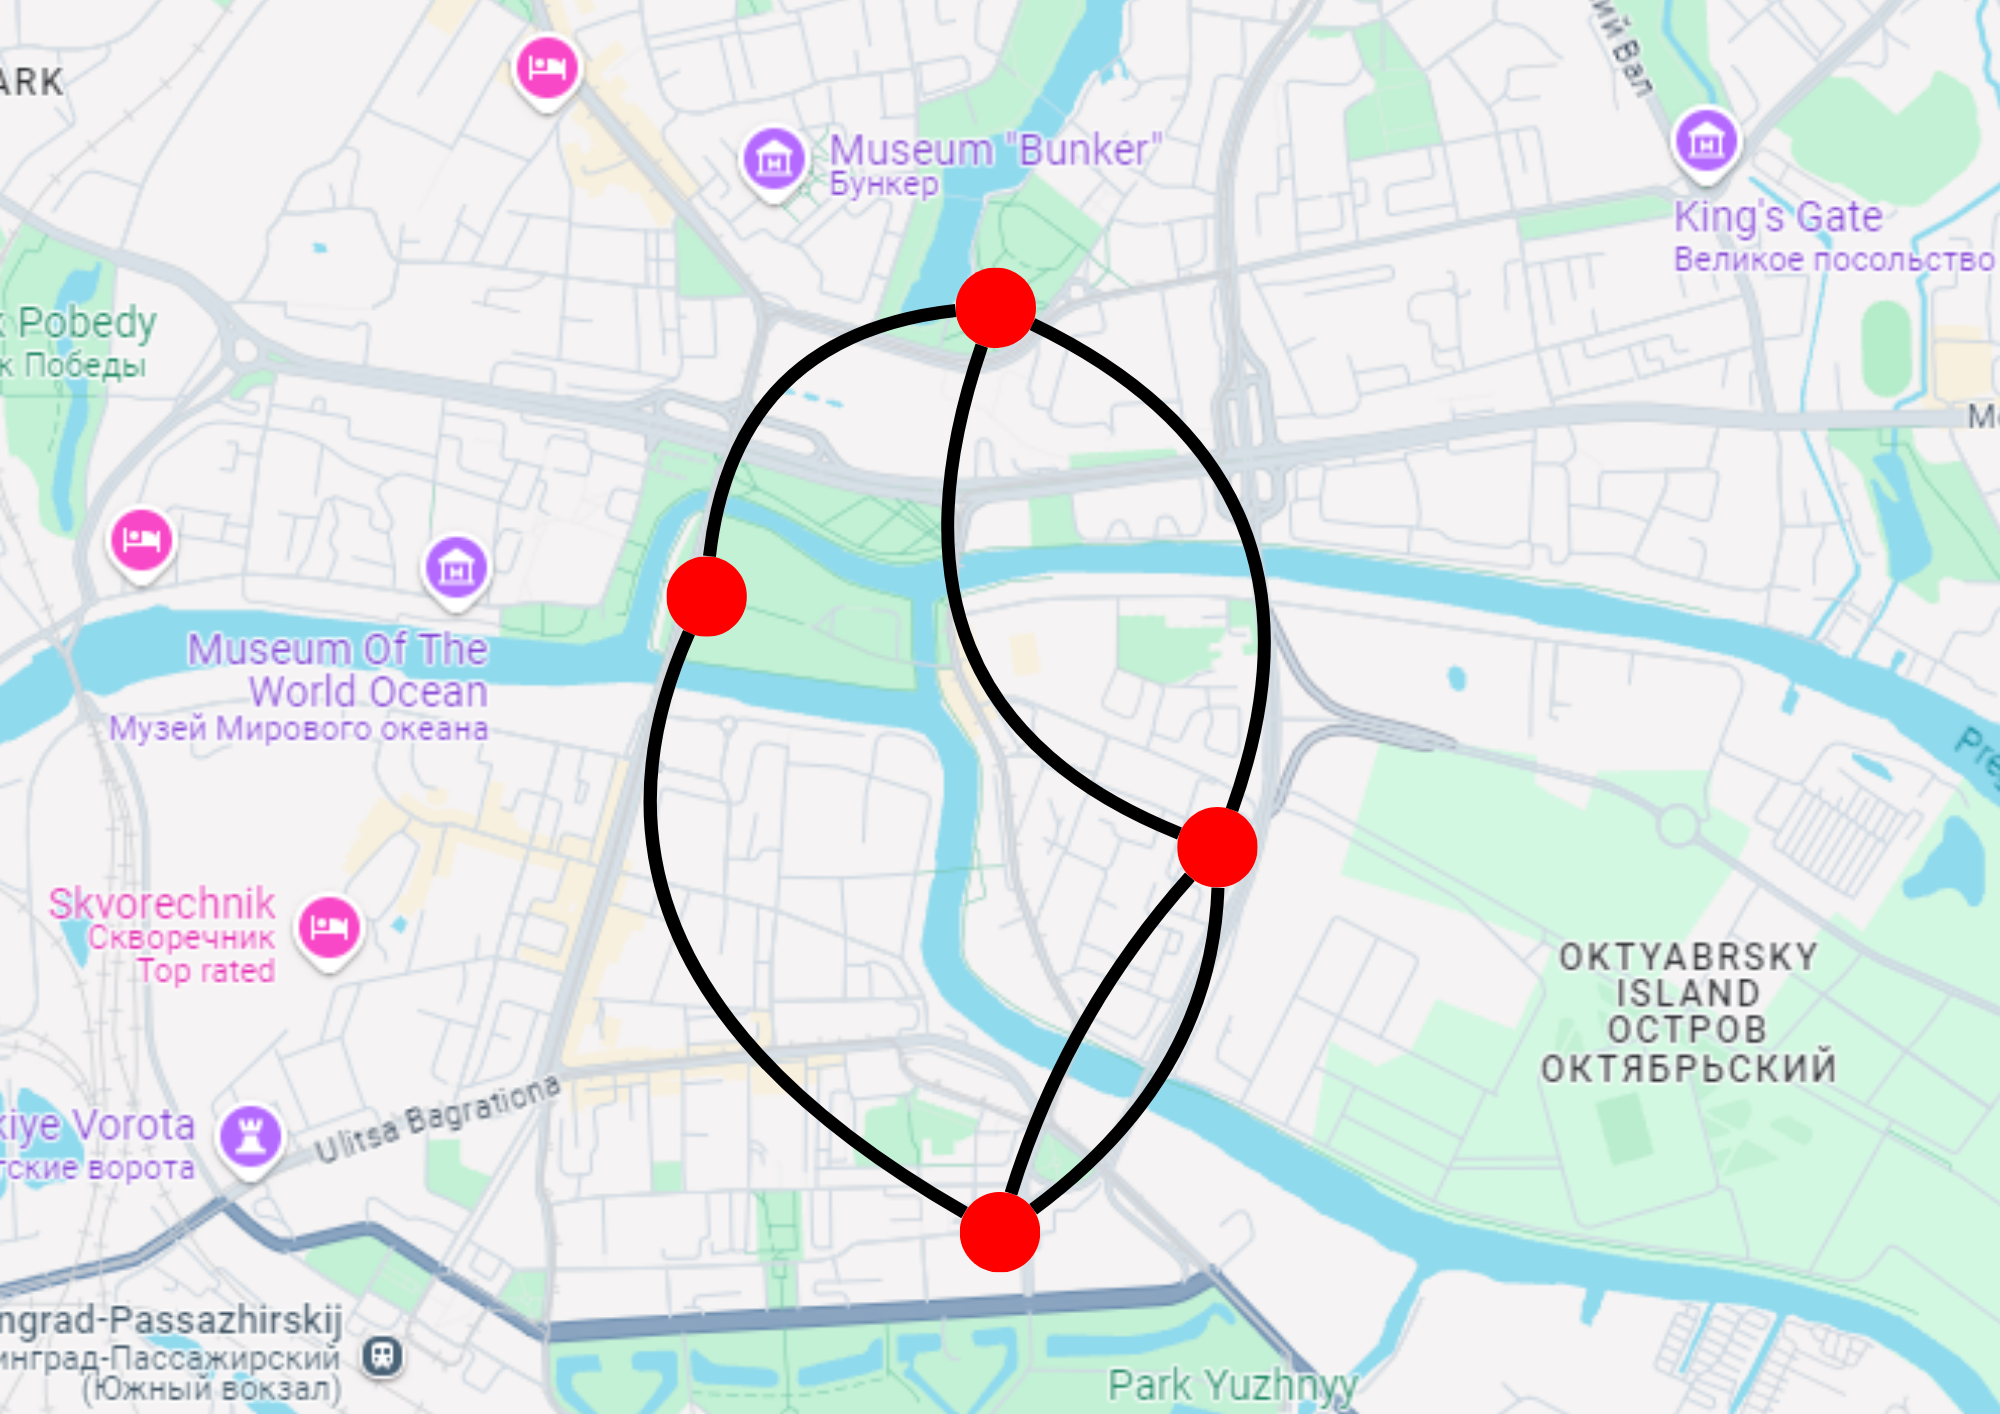
\includegraphics[width=0.5\linewidth]{gambar/Graf Konigsberg.png}
        \vspace{5mm}
        \caption{Graf Representasi "Tujuh Jembatan K$\ddot{o}$nigsberg"}
        \label{gam:Graf Konigsberg}
    \end{figure}

    % Sub-Subbab
    \vspace{-5mm}
    \subsection{Definisi Graf}
    {\frenchspacing
        Terminologi dari sebuah graf dapat memiliki makna yang berbeda akibat dari luasnya aplikasi graf pada berbagai bidang.
        Sebuah simpul dari graf pada studi kasus yang berbeda mungkin menyatakan objek yang berbeda.
        Oleh karena itu secara kasar, graf dapat dipandang sebagai suatu diagram yang memuat sejumlah informasi tertentu dari sebuah studi kasus.

        Suatu graf dinotasikan dengan $G=(V,E)$ dalam matematika memiliki definisi sebagai berikut.
        \begin{definisi}
            \label{def:Graf}
            Suatu graf $G=(V,E)$ terdiri 2 himpunan pasangan berurut yang berhingga, yaitu himpunan
            tidak kosong dari titik-titik disebut simpul atau "vertices" (dinotasikan $V(G)$) dan
            himpunan garis-garis dua elemen subset dari $V(G)$ disebut sisi atau "edges" (dinotasikan $E(G)$).
        \end{definisi}
        \noindent
        Setiap sisi di dalam graf $G$ berhubungan dengan satu atau dua simpul.
        Sisi yang terhubung hanya dengan satu simpul disebut \textit{loop}.
        Simpul di dalam graf $G$ dapat terhubung dengan lebih dari satu sisi yang berbeda.
        Dua sisi berbeda yang terhubung dengan satu simpul sama disebut sebagai garis atau sisi paralel.
        Sisi yang terhubung dengan dua simpul berbeda menyebabkan kedua simpul tersebut menjadi terhubung (\textit{adjacent}) \mycite{Jek:2016}.

        \begin{figure}
            \centering
            \begin{tikzpicture}
                \node [vertex] (A) at (0,0) {}; \node[above left] at (A) {$v_{1}$};
                \node [vertex] (B) at (2,2) {}; \node[above] at (B) {$v_{2}$};
                \node [vertex] (C) at (2.8, -0.8) {}; \node[below left] at (C) {$v_{3}$};
                \node [vertex] (D) at (4, -1.5) {}; \node[right] at (D) {$v_{4}$};

                \path [edge] (A) edge[in = 160, out = 250, min distance = 3cm] node[left] {$e_{1}$} (A);
                \path [edge] (A) -- node[midway, left] {$e_{2}$} (B);
                \path [edge] (A) -- node[midway, below] {$e_{3}$} (C);
                \path [edge] (B) -- node[midway, right] {$e_{4}$} (C);
                \path [edge] (C) edge[in = 100, out = 25, looseness = 1] node[above] {$e_{5}$} (D);
                \path [edge] (C) edge[in = 190, out = 260, looseness = 1] node[below] {$e_{6}$} (D);
            \end{tikzpicture}
            \vspace{-7mm}
            \caption{Graf G}
            \label{gam:Graf G}
        \end{figure}
    }

    % Sub-Subbab
    \vspace{-5mm}
    \subsection{Jalan, Lintasan, dan Sirkuit}
    {\frenchspacing
        Simpul-simpul di dalam graf $G$ dapat dihubungkan oleh lebih dari satu sisi.
        Jumlah sisi yang terhubung dengan suatu simpul pada graf disebut derajat simpul sesuai dalam definisi berikut.
        \begin{definisi}
            \label{def:Derajat Graf}
            Misalkan $v$ merupakan simpul dalam suatu graf $G$.
            Derajat simpul $v$ (dinotasikan $d(v)$) adalah jumlah sisi yang terhubung dengan simpul $v$
            dan sisi suatu \textit{loop} dihitung dua kali.
            Derajat total $G$ didapat dengan menjumlahkan derajat semua simpul dalam $G$.
        \end{definisi}
        \noindent
        Derajat suatu simpul dalam graf berarah dapat dinyatakan sebagai jumlahan sisi berarah masuk ke simpul dan jumlahan sisi
        berarah keluar dari simpul \mycite{Nurdiyanto:2019}.

        Barisan yang diawali dari simpul awal dan diakhiri pada simpul akhir serta
        terdapat sisi-sisi dan simpul-simpul secara selang-seling disebut jalan (\textit{walk}).
        Jalan sederhana dengan panjang $n$ dari $v_{0}$ sampai $v_{n}$ dituliskan sebagai berikut :
        $v_{0} e_{1} v_{1} \dots $ $v_{n-1} e_{n} v_{n}$.
        Jalan dapat dimulai dari simpul awal sampai dengan simpul akhir yang semua sisinya berbeda akan membuat sebuah lintasan (\textit{path}).
        Lintasan dengan simpul awal dan simpul akhir yang sama dapat disebut sebagai sirkuit (\textit{circuit}) \mycite{Rahayuningsih:2018}.
    }

    % Sub-Subbab
    \vspace{-5mm}
    \subsection{Graf Berbobot}
    {\frenchspacing
        Suatu graf berbobot (\textit{Weighted Graph}) merupakan konsep dalam teori graf dengan memberikan bobot atau
        nilai bertipe numerik terhadap sisi yang terhubung dengan dua simpul pada suatu graf.
        Bobot ini merepresentasikan suatu atribut tertentu yang terkait dengan relasi antara simpul-simpul sesuai
        dengan informasi pemanfaatan graf tersebut.
        Salah satu pemanfaatan graf berbobot dapat digunakan untuk pencarian rute terpendek dengan bobot yang mungkin
        merepresentasikan jarak, biaya transportasi, atau waktu \mycite{Pratama:2022}.
    }

    % Sub-SubBab
    \vspace{-5mm}
    \subsection{Representasi Graf Tak Berarah Dalam Matriks}
    {\frenchspacing
        Selaras dengan terminologi graf yang memiliki banyak makna bergantung pada fungsi suatu graf dalam aplikasinya,
        Suatu graf tak berarah dapat dipetakan menjadi sebuah matriks untuk merepresentasikan hubungan antar elemen-elemen dalam graf tersebut.
        Keuntungan dari merepresentasikan graf dalam matriks dapat mempermudah perhitungan yang diperlukan.
        Namun, keterbatatasan matriks untuk mencakup keseluruhan informasi pada suatu graf menjadi kesulitan utama.
        Terdapat beberapa matriks untuk menyatakan suatu graf tak berarah, diantaranya matriks ketetanggaan dan matriks ketetanggaan berbobot \mycite{Chen:2020}.

        % Anak Sub-SubBab
        \vspace{-5mm}
        \subsubsection{Matriks Ketetanggaan}
        {\frenchspacing
            Matriks ketetanggaan (\textit{adjacency matrix}) merupakan matriks yang menyatakan hubungan jumlah sisi dan simpul dari suatu graf yang didefinisikan sebagai berikut.

            \begin{definisi}
                \label{def:Matriks ketetanggaan}
                Misalkan $G$ adalah graf tak berarah dengan simpul-simpul berhingga ($n$).
                Matriks ketetanggaan yang sesuai dengan graf $G$ adalah matriks $A=(a_{ij});$ $i,j=1,2,\dots,n$ dengan $a_{ij}$ merepresentasikan jumlah sisi yang menghubungkan antar simpul yang terhubung.
            \end{definisi}

            \noindent
            Perhatikan pada graf tak berarah bahwa jumlah sisi yang menghubungkan simpul $v_{i}$ ke simpul $v_{j}$ selalu sama
            dengan jumlah sisi yang menghubungkan simpul $v_{j}$ ke simpul $v_{i}$.
            Akibatnya, matriks ketetanggaan yang merepresentasikan graf tak berarah selalu merupakan matriks yang simetris \mycite{Jek:2016}.

            \begin{contoh}
                \label{con:Matriks ketetanggaan}
                Diberikan suatu graf $G$ tak berarah sebagai $G=(\{v_{1},v_{2},v_{3}\},\{(v_{1},v_{1}),$ $(v_{1},v_{2}),(v_{1},v_{2}),(v_{1},v_{3})\})$.
                Nyatakan graf $G$ ke dalam bentuk matriks!

                \begin{figure}\label{gam:Contoh Matriks Ketetanggaan}
                    \centering
                    \begin{tikzpicture}
                        \node [vertex] (A) at (0,0) {}; \node[above left] at (A) {$v_{1}$};
                        \node [vertex] (B) at (2,2) {}; \node[above] at (B) {$v_{2}$};
                        \node [vertex] (C) at (3,-0.5) {}; \node[below right] at (C) {$v_{3}$};

                        \path [edge] (A) edge[in = 180, out = 270, looseness = 30] node[left] {$e_{1}$} (A);
                        \path [edge] (A) edge[in = 190, out = 90, looseness = 1] node[above left] {$e_{2}$} (B);
                        \path [edge] (A) edge[in = 280, out = 15, looseness = 1] node[below] {$e_{3}$} (B);
                        \path [edge] (A) -- node[midway, below] {$e_{4}$} (C);
                    \end{tikzpicture}
                    \vspace{-7mm}
                    \caption{Graf Contoh \ref{con:Matriks ketetanggaan}}
                \end{figure}

                \noindent
                \textbf{Penyelesaian:}

                {\noindent
                    Matriks ketetanggaan yang merepresentasikan graf $G$ adalah sebagai berikut.

                    \begin{equation*}
                        M_{G} =
                        \begin{bNiceArray}{ccc}[first-row,first-col]
                            & v_{1} & v_{2} & v_{3} \\
                            v_{1} & 1     & 2     & 1     \\
                            v_{2} & 2     & 0     & 0     \\
                            v_{3} & 1     & 0     & 0
                        \end{bNiceArray}
                    \end{equation*}
                }
            \end{contoh}

            Misal suatu graf tak berarah $G$ memiliki bobot pada setiap sisinya, maka matriks ketetanggaan menyatakan bobot dari simpul yang terhubung kemudian
            disebut sebagai matriks ketetanggaan berbobot (\textit{weighted adjacency matrix}). Matriks ketetanggaan berbobot yang merepresentasikan graf tak berarah
            akan bernilai $0$ jika simpul-simpul tersebut tidak terhubung \mycite{Akhirina:2020}.

            \begin{contoh}
                \label{con:Matriks Ketetanggaan Berbobot}
                Diberikan suatu graf $G$ tak berarah berbobot direpresentasikan dalam gambar berikut.

                \begin{figure}
                    \centering
                    \begin{tikzpicture}
                        \node [vertex] (A) at (0,0) {}; \node[below right] at (A) {$v_{1}$};
                        \node [vertex] (B) at (2,2) {}; \node[above right] at (B) {$v_{2}$};
                        \node [vertex] (C) at (3,0.6) {}; \node[below right] at (C) {$v_{3}$};

                        \path [edge] (A) edge[in = 110, out= 200, looseness = 30] node[above left] {$5$} (A);
                        \path [edge] (A) -- node[midway, above left] {$7$} (B);
                        \path [edge] (A) -- node[midway, below] {$9$} (C);
                        \path [edge] (B) -- node[midway, above right] {$9$} (C);
                    \end{tikzpicture}
                    \vspace{0mm}
                    \caption{Graf Contoh \ref{con:Matriks Ketetanggaan Berbobot}}
                    \label{gam:Contoh Matriks ketetanggaan Berbobot}
                \end{figure}

                \noindent
                Nyatakan graf $G$ ke dalam matriks ketetanggaan berbobot!

                \noindent
                \textbf{Penyelesaian:}

                {\noindent
                    Matriks ketetanggaan berbobot yang merepresentasikan graf $G$ sebagai berikut.

                    \begin{equation*}
                        A_{G} =
                        \begin{bNiceArray}{ccc}[first-row,first-col]
                            & v_{1} & v_{2} & v_{3} \\
                            v_{1} & 5 & 7 & 9 \\
                            v_{2} & 7 & 0 & 9 \\
                            v_{3} & 9 & 9 & 0
                        \end{bNiceArray}
                    \end{equation*}

                }
            \end{contoh}

            Apabila suatu graf $G$ tak berarah memiliki dua simpul ($v_{1}$ dan $v_{2}$) dihubungkan oleh dua sisi dengan bobot berbeda,
            maka representasi matriks ketetanggaan berbobot untuk dua simpul tersebut menyesuaikan pengaplikasiannya. Graf tak berarah yang merepresentasikan
            permasalahan maksimasi akan mengambil bobot dengan nilai terbesar dan berlaku sebaliknya.
        }

        % Sub-SubBab
        \vspace{-5mm}
        \subsubsection{Matriks Biner}
        {\frenchspacing
            Matriks biner dapat juga disebut matriks ($0-1$) atau matriks insidensi (\textit{incidence matrix}) adalah matriks
            yang menyatakan hubungan keterhubungan simpul dengan sisi dari suatu graf yang didefinisikan sebagai berikut.
            \begin{definisi}
                \label{def:Definisi Matriks Biner}
                Misalkan $G$ adalah graf tanpa loop dengan $n$ simpul $v_{1},v_{2},\dots,v_{n}$ dan $k$ sisi $e_{1},e_{2},\dots,e_{k}$.
                Matriks biner yang sesuai dengan graf $G$ adalah matriks $A$ berukuran $n\times k$ yang elemennya terdiri dari

                \begin{equation}
                    a_{ij} = \begin{cases} 1 & ,\text{jika simpul $v_{i}$ berhubungan dengan sisi $e_{j}$} \\ 0 &,,\text{jika simpul $v_{i}$ tidak berhubungan dengan sisi $e_{j}$} \end{cases}
                    \label{pers:Definisi Matriks Biner}
                \end{equation}

            \end{definisi}
            \noindent
            Matriks biner sering digunakan ke dalam bidang teori kode, logika digital, dan operasi komputasi \mycite{Jek:2016}.
        }
    }
}
\vspace{-3mm}

% SubBab
\section{Optimasi}
\vspace{-4mm}
{\frenchspacing
    Optimasi atau optimalisasi merupakan suatu prinsip pencarian solusi layak yang bersifat tepat, efektif, dan efisien (optimum) \mycite{Atiqoh:2020}.
    Pengertian teknis dari optimasi dapat diartikan sebagai tindakan tersistematis yang memaksimalkan sumber daya yang tersedia
    dengan tujuan menemukan solusi optimal.
    Solusi dalam optimasi berada dalam daerah layak (\textit{feasible region}) yang memiliki nilai minimum atau maksimum dari fungsi objektif.
    Proses pencarian solusi optimum dalam optimasi terkait dengan permasalahan komputasional yang bertujuan
    menemukan solusi terbaik dan layak dari sejumlah alternatif solusi terbatas.
    Penerapan optimasi sering diterapkan dalam banyak permasalahan yang memiliki keterbatasan sumber daya,
    seperti permasalahan pencarian rute terpendek pada konsep \textit{traveling salesman problem} (TSP) \mycite{Riri:2020}.
}
\vspace{-3mm}

% SubBab
\section{Konsep \textit{Traveling Salesman Problem} (TSP)}
\vspace{-4mm}
{\frenchspacing
    \textit{Traveling salesman problem} (TSP) merupakan salah satu konsep klasik dalam teori graf
    dan kombinatorial mengenai pencarian rute terpendek atau lintasan tertutup yang mengunjungi
    setiap simpul (lokasi) tepat satu kali dan kembali ke simpul awal dengan mengoptimalkan total jarak atau
    biaya perjalanan agar minimum. Representasi suatu permasalahan TSP umumnya dimodelkan ke dalam graf
    dengan simpul sebagai lokasi dan sisi sebagai bobot yang akan dioptimalkan.
    Meskipun konsep TSP terlihat sederhana, namun tingkat kesulitan akan meningkat seiring
    eksponensial jumlah kemungkinan jalur saat jumlah simpul meningkat \mycite{Sinaga:2023}.

    Pembentukan pertama kajian matematika terhadap permasalahan TSP oleh seorang matematikawan Irlandia W.R. Hamilton pada abad ke-19.
    Penyelesaian permasalahan TSP diperoleh melalui pendekatan-pendekatan tertentu.
    Penyelesaian TSP melalui pendekatan matematis pertama oleh Merril Flood pada tahun 1930.
    Kemudian permasalahan tersebut dikenal dengan nama \textit{Traveling Salesman Problem} yang diciptakan oleh Hassler Whitney dari Universitas Princeton.
    Permasalahan TSP termasuk ke dalam permasalahan \textit{nondeterministic polynomial time-hard}(\textit{NP-Hard}) yang berarti tidak ada algoritma yang efisien untuk setiap permasalahan TSP \mycite{Kumar:2020}.

    Konsep TSP memiliki banyak penerapan praktis untuk memecahkan permasalahan optimasi yang melibatkan
    penentuan rute terpendek sehingga setiap simpul dapat dikunjungi dengan biaya atau waktu minimal.
    Pemecahan solusi optimal untuk permasalahan TSP dengan jumlah simpul yang besar akan menjadi cukup sulit.
    Pendekatan dengan berbagai metode banyak dilakukan agar dapat memperoleh solusi yang optimal,
    salah satunya adalah metode pendekatan secara heuristik \mycite{Saud:2018}.
}
\vspace{-3mm}

% SubBab
\section{Metode Heuristik}
\vspace{-4mm}
{\frenchspacing
    Metode heruistik merupakan strategi pendekatan komputasional untuk menyelesaikan
    permasalahan pengambilan keputusan yang mungkin sulit bahkan tidak mungkin diselesaikan secara eksak dalam waktu yang wajar.
    Tujuan utama dari metode heuristik adalah untuk menghasilkan solusi yang cukup baik dengan biaya komputasi yang juga terjangkau.
    Heuristik mengacu pada aturan praktis atau strategi mental berbasis pengalaman, pengetahuan, atau asumsi yang digunakan dalam mengambil keputusan dengan penyederhanaan prosesnya.
    Meskipun metode heuristik dapat membantu terhadap permasalahan yang kompleks atau tidak pasti, namun solusi yang dihasilkan tidak menjamin optimal dan sering menyebabkan bias dalam pemikiran \mycite{Anwar:2024}.

    Metode heuristik secara umum memberikan kerangka kerja yang sederhana dan cepat dengan berbasis pengalaman dan pengetahuan.
    Adapun beberapa metode heuristik secara umum adalah sebagai berikut:
    \begin{enumerate}[align=left, left = 0mm, nolistsep]
        \item Heuristik Ketersediaan \par \nobreak
              Heuristik ketersediaan mengambil keputusan didasarkan pada seberapa mudah mengingat kembali contoh-contoh atau informasi terkait.
              Contohnya orang yang baru mendengar kabar mengerikan mengenai kecelakaan kapal akan berpikir bahwa berlayar itu pilihan tidak aman.
        \item Heuristik Representatif \par \nobreak
              Heuristik representatif mengambil keputusan didasarkan pada asumsi suatu objek atau kondisi serupa dengan pola atau kategori tertentu seperti kesamaan fitur atau kesamaan karakteristik lain.
              Contohnya penampilan seseorang dinilai mewakili karakteristik kelompok tertentu.
        \item Heuristik Ancoran dan Penyesuaian \par \nobreak
              Heuristik estimasi awal (ancoran) dan penyesuaian mengambil keputusan dengan membuat estimasi awal berdasarkan informasi awal yang kemudian mengubah estimasi tersebut berdasarkan informasi yang diterima selanjutnya.
              Contohnya tawar-menawar harga mobil dengan estimasi awal mengikuti harga jual awal oleh penjual kemudian berubah berdasarkan informasi spesifikasi mobil tersebut.
        \item Heuristik Kesederhanaan \par \nobreak
              Heuristik kesederhanaan mengambil keputusan secara sederhana berdasarkan pada informasi yang paling mudah diakses untuk menggantikan informasi sebenarnya.
              Contohnya memutuskan membeli sepatu merk A menggunakan opini yang sedang \textit{trending} di media sosial.
        \item Heuristik Atribusi \par \nobreak
              Heuristik atribusi mengambil keputusan didasarkan pengetahuan saat ini untuk memberikan penjelasan singkat terhadap kondisi atau perilaku tertentu.
              Contohnya memberikan penjelasan bahwa orang yang terlambat itu akibat dari rasa malas dari orang tersebut.
    \end{enumerate}

    \noindent
    Metode heuristik banyak diaplikasikan ke dalam berbagai bidang yang dihadapkan pengambilan keputusan tertentu.
    Salah satu contoh penggunaan metode heuristik adalah algoritma \textit{particle swarm optimization} yang termasuk ke dalam metode heuristik representatif dengan menggunakan
    perilaku sosial kawanan hewan dalam mencari mangsa sebagai representatif permasalahan optimasi \mycite{Muhammad:2023}.
}
\vspace{-3mm}

% SubBab
\section{Algoritma \textit{Particle Swarm Optimization} (PSO)}
\vspace{-4mm}
{\frenchspacing
Algoritma \textit{particle swarm optimization} (PSO) merupakan algoritma optimasi heurisitik berbasis populasi yang diperkenalkan oleh James Kennedy dan Russel Eberhart pada tahun 1995.
Basis populasi terinspirasi dari perilaku sosial hewan seperti burung dalam suatu kawanan (\textit{swarm}) pada saat menelusuri area tertentu untuk mencari makanan.
Perilaku sosial kawanan tersebut dalam mencari makanan meliputi kecerdasan, kecepatan, dan komunikasi yang terorganisir \mycite{Kusrahman:2020}.

% Sub-SubBab
\vspace{-5mm}
\subsection{Definisi Algoritma \textit{Particle Swarm Optimization}}
{\frenchspacing
    Algoritma \textit{particle swarm optimization} merupakan salah satu teknik optimasi komputasional.
    Perilaku sosial hewan dalam mencari makan pada suatu daerah menginspirasi konsep dasar algoritma \textit{particle swarm optimization}.
    Konsep untuk mengeksploitasi individu dalam pencarian solusi, dilakukan dengan populasi yang disebut \textit{swarm} dan individu disebut \textit{particle}.
    Setiap \textit{particle} akan bergerak semakin mendekati solusi dengan kecepatan (\textit{velocity}) yang terus beradaptasi terhadap daerah pencarian
    dan informasi posisi terbaik yang pernah dicapai selalu disimpan \mycite{Muhammad:2023}.

    Konsep penelusuran algoritma \textit{particle swarm optimization} memiliki kesamaan dengan algoritma genetika, yaitu populasi awal yang digunakan adalah populasi acak dalam bentuk matriks.
    Representasi populasi pada matriks menggunakan baris sebagai \textit{particle} untuk algoritma \textit{particle swarm optimization} atau kromosom untuk algoritma genetika.
    Perbedaan mendasar antara kedua algoritma ini adalah algoritma \textit{particle swarm optimization} tidak memiliki operator yang dapat mengevolusi partikel seperti \textit{crossover} dan mutasi pada algoritma genetika \mycite{Zahro:2020}.

    Algoritma \textit{particle swarm optimization} menggunakan beberapa istilah untuk mencakup informasi dari suatu persamalahan optimasi.
    Adapun istilah umum yang sering digunakan dalam algoritma \textit{particle swarm optimization} dijelaskan sebagai berikut:
    \begin{enumerate}[align=left, left=0em, nolistsep]
        \item \textit{Swarm} : populasi dari algoritma \textit{particle swarm optimization}.
        \item \textit{Particle} $(X_{j})$ : individu di dalam suatu \textit{swarm}.
              Dalam satu terdiri dari beberapa dimensi $(d)$ sesuai dengan dimensi dari model permasalahan yang akan diselesaikan.
              Seluruh \textit{particle} merepresentasikan solusi potensial pada saat proses optimisasi.
              Posisi setiap \textit{particle} selalu diperbarui berdasarkan kecepatan (\textit{velocity}) tertentu.
        \item \textit{Velocity} (\textbf{$v$}): vektor yang memperbarui posisi dan arah \textit{particle} berpindah dari posisi semula.
        \item \textit{Inertia Weight} ($\omega$) : parameter untuk mengendalikan dampak dari \textit{velocity} sebelumnya terhadap \textit{velocity} sekarang suatu \textit{particle}.
        \item \textit{Personal Best} ($P_{best}$) : posisi terbaik yang pernah dicapai oleh \textit{particle} yang dipersiapkan untuk mendapatkan solusi terbaik.
        \item \textit{Global Best} ($G_{best})$ : posisi terbaik \textit{particle} pada \textit{swarm}.
    \end{enumerate}
    \begin{rightcite}
        \mycite{Muhardeny:2023}.
    \end{rightcite}

    Partikel solusi dalam algoritma \textit{particle swarm optimization} diperoleh dari partikel dengan posisi yang menghasilkan nilai fungsi \textit{fitness} terbaik di semua iterasi.
    Partikel berisikan posisi dari sejumlah dimensi partikel, dimana dimensi partikel merupakan jumlah parameter yang akan dioptimalkan.
    Proses pencarian solusi pada algoritma \textit{particle swarm optimization} memandang bahwa untuk setiap partikel cenderung akan bergerak ke arah solusi berdasarkan kecepatan (\textit{velocity}).
    Vektor posisi dan kecepatan partikel pada iterasi sekarang dapat dinotasikan dalam persamaan berikut:

    \begin{equation}
        \textbf{\textit{X}}_{j}^{(i)} = \begin{bmatrix} x_{j,1}^{(i)} \\ \vdots \\ x_{j,d}^{(i)} \end{bmatrix}
        \label{pers: Vektor Posisi}
    \end{equation}

    \noindent
    dan

    \begin{equation}
        \textbf{\textit{V}}_{j}^{(i)} = \begin{bmatrix} v_{j,1}^{(i)} \\ \vdots \\ v_{j,d}^{(i)} \end{bmatrix}
        \label{pers: Vektor Kecepatan}
    \end{equation}

    \noindent
    dengan $j$ adalah indeks dari partikel dan $d$ adalah jumlah dimensi partikel \mycite{Akpudo:2020}.

    Penggunaan algoritma \textit{particle swarm optimization} memiliki keuntungan utama yaitu memiliki waktu komputasi yang rendah, parameter yang perlu disesuaikan relatif sedikit, dan
    mampu membangun model matematika yang akurat untuk suatu permasalahan kompleks.
    Keuntungan lain penggunaan algoritma \textit{particle swarm optimization} adalah tidak terjadi tumpah tindih atau mutasi pada saat proses perhitungan.
    Keuntungan tersebut sudah cukup menjadikan algoritma \textit{particle swarm optimization} sering untuk digunakan.
    Namun algoritma ini memiliki kelemahan, salah satunya adalah memerlukan penyimpanan data lebih untuk memperbarui \textit{velocity} maupun posisi terbaik saat iterasi \mycite{Gad:2022}.
}

% Sub-SubBab
\vspace{-5mm}
\subsection{Parameter Algoritma \textit{Particle Swarm Optimization}}
{\frenchspacing
    Parameter dalam algoritma \textit{particle swarm optimization} memberikan pengaruh besar terhadap kinerja algoritma.
    Pemilihan parameter yang digunakan dan penentuan nilainya dapat meningkatkan kinerja algoritma menjadi lebih efisien.
    Terdapat beberapa parameter dasar dari algoritma \textit{particle swarm optimization} dijelaskan sebagai berikut:
    \begin{enumerate}[align=left, left=0em, nolistsep]
        \item Ukuran \textit{Swarm} \par \nobreak
              Ukuran \textit{swarm} merupakan nilai banyaknya \textit{swarm} yang menjadi populasi dari algoritma.
              Penentuan ukuran \textit{swarm} yang besar dapat mengurangi jumlah iterasi untuk mencapai perhitungan yang konvergen.
              Akan tetapi, penggunaan ukuran \textit{swarm} yang besar tentu akan meningkatkan perhitungan tiap iterasi menjadi lebih kompleks.
              Hal ini mengakibatkan waktu untuk menyelesaikan perhitungan dalam satu iterasi menjadi semakin lama.
              Besar dari sebuah populasi juga dapat menentukan ukuran \textit{swarm}.
              Beberapa penelitian tentang implementasi algoritma \textit{particle swarm optimization} klasik menggunakan
              interval $N \in [20,50]$ untuk ukuran \textit{swarm} \mycite{Piotrowski:2020}.
        \item Jumlah iterasi \par \nobreak
              Jumlah iterasi merupakan jumlah pengulangan dari proses perhitungan yang akan dilakukan dalam algoritma.
              Penentuan jumlah iterasi pada algoritma \textit{particle swarm optimization} mempengaruhi pencarian solusi optimal.
              Jika jumlah iterasi yang digunakan terlalu kecil akan berdampak pada proses perhitungan menjadi berhenti saat solusi belum mencapai optimal.
              Namun sebaliknya, jumlah iterasi yang terlalu besar akan menyebabkan proses perhitungan menjadi semakin kompleks, menambah waktu perhitungan, serta
              menambahkan perhitungan yang tidak diperlukan \mycite{Meetu:2022}.
        \item \textit{Learning Rates} ($c_{1}$ dan $c_{2}$) \par \nobreak
              \textit{Learning rates} atau \textit{acceleration coefficients} terdiri dari dua parameter adaptif dalam algoritma \textit{particle swarm optimization} yang mengatur keseimbangan dari kecerdasan posisi partikel
              terhadap pengalaman pribadi yaitu $(P_{best})$ dan pengalaman kolektif yaitu $(G_{best})$.
              Parameter koginitf $(c_{1})$ merupakan parameter yang mengatur pengaruh $P_{best}$ terhadap posisi partikel.
              Sedangkan, parameter sosial $(c_{2})$ merupakan parameter yang mengatur pengaruh $G_{best}$ terhadap posisi partikel.
              Terdapat beberapa penentuan nilai $c_{1}$ dan $c_{2}$, yaitu sebagai berikut:

              \begin{enumerate}[label=(\alph*)., align=left, left=0em, nolistsep]
                  \item Jika $c_{1}=c_{2}=0$, maka setiap partikel akan bergerak dengan kecepatan partikel tersebut secara konstan sampai batas ruang pencarian.
                  \item Jika $c_{1}>0$ dan $c_{2}=0$, maka setiap partikel akan bergerak dengan kecepatan partikel terhadap $P_{best}$ masing-masing (independen) karena komponen sosial tidak mempengaruhi.
                        Sedangkan sebaliknya, maka setiap partikel akan bergerak dengan kecepatan partikel terhadap $G_{best}$ sehingga partikel hanya akan tertarik pada satu arah titik.
                  \item Jika $c_{1}=c_{2}$, maka setiap partikel akan bergerak dengan kecepatan partikel terhadap rata-rata dari $P_{best}$ dan $G_{best}$.
                  \item Jika $c_{1}>c_{2}$, maka kecepatan partikel untuk setiap partikel akan lebih dipengaruhi oleh $P_{best}$ daripada $G_{best}$.
                        Sedangkan sebaliknya, maka kecepatan partikel akan lebih dipengaruhi $G_{best}$ daripada $P_{best}$.
              \end{enumerate}

              Penentuan nilai dari $c_{1}$ dan $c_{2}$ secara umum bersifat statis yang diperoleh dari beberapa penelitian terhadulu.
              Kesalahan dalam penentuan nilai $c_{1}$ dan $c_{2}$ menyebabkan proses pencarian solusi menjadi divergen.
              Dalam berbagai penelitian, telah diusulkan bahwa penentuan nilai $c_{1}$ dan $c_{2}$ dapat menggunakan nilai $c_{1}=c_{2}=2$ \mycite{Meetu:2022}.
        \item \textit{Inertia Weight} ($\omega$) \par \nobreak
              \textit{Inertia weight} atau bobot inersia $(\omega)$ merupakan parameter yang mengontrol efek dari \textit{velocity} sebelumnya terhadap \textit{velocity} sekarang dari suatu partikel.
              Penentuan \textit{inertia weight} yang terlalu besar akan menyebabkan peningkatan berlebihan pada \textit{velocity} saat diperbarui, akibatnya partikel akan terlalu jauh bergerak dan terlalu cepat bahkan melewati solusi optimal.
              Terdapat beberapa penentuan nilai \textit{inertia weight}, yaitu sebagai berikut:

              \begin{enumerate}[label=(\alph*)., align=left, left=0em, nolistsep]
                  \item Jika $\omega \geq 1$, maka nilai \textit{velocity} akan meningkat secara berlebih saat diperbarui dan tidak dapat bergerak ke arah yang optimal sehingga solusi akan menjadi divergen.
                  \item Jika $\omega < 1$, maka akan terdapat momentum kecil pada \textit{velocity} sebelumnya sehingga dapat digunakan untuk melakukan perubahan arah secara cepat menuju ke posisi yang lebih baik saat proses pencarian solusi.
                  \item Jika $\omega = 0$, maka partikel akan bergerak tanpa mengetahui \textit{velocity} sebelumnya sehingga partikel tidak dapat mengetahui perubahan posisinya secara benar bahkan dapat keluar dari arah solusi optimal.
              \end{enumerate}

              Nilai \textit{inertia weight} yang sesuai dengan ketentuan tersebut adalah pada interval $\omega \in [0.1, 0.9]$.
              Shi dan Eberhart memperkenalkan strategi \textit{constant inertia weight} dan \textit{random inertia weight}.
              Strategi \textit{constant inertia weight} akan mengambil nilai \textit{inertia weight} di setiap iterasi adalah konstan $(\omega^{(i)} = \omega)$.
              Sedangkan pada strategi \textit{random inertia weight}, nilai \textit{inertia weight} diambil secara acak namun tetap berada
              di atas rata-rata dari interval ketentuan. Nilai \textit{inertia weight} di setiap iterasi $i$ dengan strategi \textit{random inertia weight} ditentukan menggunakan persamaan berikut:

              \begin{equation}
                  \omega^{(i)} = 0.5 + \frac{r}{2}
                  \label{pers: random inertia weight}
              \end{equation}

              dengan nilai $r$ adalah bilangan acak berdistribusi \textit{uniform} $r \sim{U(0,1)}$ \mycite{Zdiri:2021}.
    \end{enumerate}
}

% Sub-SubBab
\vspace{-5mm}
\subsection{Kecepatan Partikel (\textit{Velocity})}
{\frenchspacing
\textit{Velocity} atau kecepatan partikel $(v)$ merupakan vektor yang memperbarui posisi dan arah \textit{particle} berpindah dari posisi sebelumnya.
Penentuan \textit{velocity} yang terlalu besar dapat menyebabkan \textit{particle} bergerak tidak menentu dan melewati solusi optimal.
Dan sebaliknya, \textit{velocity} yang terlalu kecil dapat menyebabkan \textit{particle} bergerak terlalu lambat bahkan tidak bergerak sehingga
posisinya terjebak hanya di lokal optimal. Eberhart dan Kennedy pertama kali memperkenalkan strategi batas penentuan kecepatan (\textit{velocity clamping}).
Strategi \textit{velocity clamping} menentukan kecepatan maksimum $(V_{max})$ berdasarkan inisialisasi posisi dan konstanta acak.
Kecepatan maksimum ditentukan menggunakan persamaan berikut:

\begin{equation}
    V_{max} = \varepsilon (X_{max}-X_{min})
    \label{pers: velocity clamping}
\end{equation}

\hspace{-0.675cm}dengan nilai $\varepsilon$ adalah interval nilai acak $\varepsilon \in [0,1]$ dan $X_{max},X_{min}$ adalah batas atas dan bawah dari inisialisasi posisi $(X)$ \mycite{Wang:2022}.
}

% Sub-SubBab
\vspace{-5mm}
\subsection{\textit{Personal Best}}
{\frenchspacing
    \textit{Personal best} atau lokal optimum $(P_{best})$ dalam algoritma \textit{particle swarm optimization} merupakan vektor yang menyimpan posisi terbaik untuk setiap partikel $X_{j}$ di setiap iterasi $i$.
    Posisi terbaik didasarkan pada posisi dari $X_{j}$ yang menghasilkan nilai fungsi \textit{fitness} terbaik yang pernah dicapai di semua iterasi sampai iterasi terakhir $i=n$.
    Untuk setiap iterasi, hasil perhitungan nilai fungsi \textit{fitness} partikel $X_{j}$ sekarang akan dibandingkan dengan nilai fungsi \textit{fitness} menggunakan posisi dari $P_{best}$ sebelumnya.
    Dengan kata lain, \textit{personal best} berisikan semua posisi terbaik yang pernah dikunjungi oleh partikel $X_{j}$ hingga iterasi ke $n$.
    \textit{Personal best} dapat dinotasikan sebagai berikut:

    \begin{equation}
        \textbf{\textit{P}}_{best,j}^{(i)} = \begin{bmatrix} p_{j,1}^{(i)} \\ \vdots \\ p_{j,d}^{(i)} \end{bmatrix} \in X_{j}
        \label{pers: Pbest}
    \end{equation}

    \noindent
    dengan $d$ adalah jumlah dimensi di dalam $X_{j}$ \mycite{Ramadhan:2023}.
}

% Sub-SubBab
\vspace{-5mm}
\subsection{\textit{Global Best}}
{\frenchspacing
    \textit{Global best} atau global optimum $\left(G_{best}\right)$ dalam algoritma \textit{particle swarm optimization} merupakan vektor yang menyimpan
    posisi dari $P_{best}$ terbaik saat iterasi sekarang.
    Untuk setiap iterasi $i$, $G_{best}$ didasarkan pada $P_{best}$ dari setiap partikel $X_{j}$ pada iterasi $i$ yang memiliki nilai fungsi \textit{fitness} terbaik.
    Dengan kata lain, \textit{global best} berisikan posisi dari $P_{best}$ terbaik pada iterasi sekarang.
    \textit{Global best} dapat dinotasikan sebagai berikut:

    \begin{equation}
        \textbf{\textit{G}}_{best}^{(i)} = \begin{bmatrix} g^{(i)}_{1} \\ \vdots \\ g^{(i)}_{d} \end{bmatrix}
        \label{pers: Gbest}
    \end{equation}

    \noindent
    dengan $d$ adalah jumlah dimensi di dalam $X$ \mycite{Darmawan:2022}.
}

% Sub-SubBab
\vspace{-5mm}
\subsection{Pembaruan Posisi dan \textit{Velocity}}
{\frenchspacing
Proses pencarian solusi pada algoritma \textit{particle swarm optimization} memandang bahwa setiap partikel cenderung akan bergerak
ke arah solusi berdasarkan kecepatan (\textit{velocity}) tertentu.
Posisi dan \textit{velocity} dari partikel akan selalu diperbarui di setiap iterasi sampai iterasi terakhir $i=n$.
Nilai dari \textit{velocity} akan menentukan arah perpindahan dari setiap partikel di setiap iterasi $i$ agar dapat menemukan ruang solusi terbaik.
Dalam pembaruan nilai \textit{velocity} akan terpengaruh oleh \textit{velocity}, \textit{personal best}, dan \textit{global best} dari iterasi sebelumnya.
Pembaruan posisi dan \textit{velocity} ditentukan menggunakan persamaan berikut:

\begin{equation}
    \label{pers: velocity update}
    \textbf{\textit{V}}_{j}^{(i)} = \omega^{(i)} \textbf{\textit{V}}_{j}^{(i-1)} + c_{1}r_{1}^{(i)}\left(\textbf{\textit{P}}_{best,j}^{(i-1)} - \textbf{\textit{X}}_{j}^{(i-1)}\right) + c_{2}r_{2}^{(i)} \left(\textbf{\textit{G}}_{best}-\textbf{\textit{X}}_{j}^{(i-1)}\right)
\end{equation}

\noindent
dan

\begin{equation}
    \label{pers: position update}
    \textbf{\textit{X}}_{j}^{(i)} = \textbf{\textit{X}}_{j}^{(i-1)} + \textbf{\textit{V}}_{j}^{(i)}
\end{equation}

\noindent
dengan $r_{1}^{(i)},r_{2}^{(i)}$ adalah bilangan acak berdistribusi \textit{uniform} $r \sim U(0,1)$ di setiap iterasi $i$ \mycite{Chafi:2021}.
}

% Sub-SubBab
\vspace{-5mm}
\subsection{Tahapan Algoritma \textit{Particle Swarm Optimization}}
{\frenchspacing
    Proses pencarian solusi optimum pada algoritma \textit{particle swarm optimization} dilakukan hingga iterasi maksimum atau kriteria pemberhentian terpenuhi.
    Untuk setiap iterasi, perpindahan posisi selalu diperbarui sehingga mendekati solusi optimum.
    Tahapan dan proses perhitungan algoritma \textit{particle swarm optimization} untuk konsep \textit{traveling salesman problem} sebagai berikut:

    \begin{enumerate}[align = left, left = 0cm, nolistsep]
        \item Menginisialisasi nilai parameter algoritma \textit{particle swarm optimization} seperti jumlah iterasi maksimum $(n)$, ukuran \textit{swarm} $(N)$, $(d)$, $(c_{1},c_{2})$,
              batas posisi $(X_{min},X_{max})$, posisi awal $(X_{i})$, batas \textit{velocity} maksimum $(V_{max})$, dan \textit{velocity} awal $(V_{j}^{0})$.
              Inisialisasi nilai awal dapat dilakukan melalui tahap berikut:

              \begin{enumerate}[label = (\alph*)., align = left, left = 0mm, nolistsep]
                  \item Menentukan jumlah iterasi maksimum $(n)$.
                  \item Menentukan ukuran \textit{swarm} $(N)$ dan dimensi partikel $(d)$ didasarkan pada beberapa penelitian tentang implementasi algoritma \textit{particle swarm optimization} klasik yaitu menggunakan interval $N\in[20,50]$ serta besar dimensi partikel menyesuaikan dari model permasalahan yang akan diselesaikan \mycite{Piotrowski:2020}.
                  \item Menentukan \textit{learning rates} $(c_{1})$ dan $(c_{2})$ didasarkan pada beberapa penelitian tentang \textit{learning rates} dalam algortima \textit{particle swarm optimization} yaitu menggunakan nilai $c_{1} = c_{2} = 2$ \mycite{Meetu:2022}.
                  \item Menentukan batas atas $(X_{max})$ dan batas bawah $(X_{min})$ untuk posisi partikel.
                  \item Menentukan batas \textit{velocity} maksimum $(V_{max})$ diperoleh secara acak ber-dasarkan persamaan \ref{pers: velocity clamping}, sedangkan \textit{velocity} minimum $(V_{min})$ diperoleh dari $V_{min} = - V_{max}$.
                  \item Membangkitkan \textit{velocity} awal $(\boldsymbol{V}_{j}^{0})$ sejumlah $N$ partikel secara acak yang tetap berada di batas \textit{velocity} menggunakan persamaan berikut:

                        \begin{equation}
                            v_{j,d}^{(0)} = U(V_{min},V_{max})
                            \label{pers: bangkitkan velocity awal}
                        \end{equation}

                  \item Membangkitkan posisi awal $(\boldsymbol{X}_{J}^{0})$ sejumlah $N$ partikel secara acak yang tetap berada di batas posisi partikel menggunakan persamaan berikut:

                        \begin{equation}
                            \label{pers: bangkitkan posisi awal}
                            x_{j,d}^{(0)} = U(X_{min},X_{max})
                        \end{equation}

                  \item Mengevaluasi hasil rute setiap partikel berdasarkan urutan dimensi dalam partikel dengan nilai posisi terkecil hingga terbesar.
              \end{enumerate}

        \item Mengevaluasi nilai fungsi \textit{fitness} hasil rute setiap partikel dengan menggunakan persamaan berikut:

              \begin{equation}
                  \label{pers: nilai fungsi fitness}
                  F(X_{j}^{(i)}) = \frac{1}{f(X_{j}^{(i)})}
              \end{equation}

              dengan $f(X_{j})$ adalah total biaya yang dikeluarkan untuk menggunakan hasil rute dari partikel $j$.
        \item Menentukan $P_{best}^{(0)}$ dan $G_{best}^{(0)}$ awal.
        \item Membangkitkan nilai \textit{inertia weight} berdasarkan strategi \textit{random inertia weight} menggunakan persamaan \ref{pers: random inertia weight}.
        \item Memperbarui \textit{velocity} setiap partikel menggunakan persamaan \ref{pers: velocity update} dengan nilai $r_{1}^(i)$ dan $r_{2}^(i)$ dibangkitkan secara acak menggunakan distribusi \textit{uniform} $r\sim U(0,1)$.
              Jika \textit{velocity} terbaru tidak berada di dalam batas yang diizinkan maka dilakukan penyesuaian sebagai berikut:

              \begin{equation}
                  v_{j,d}^{(i)} = \begin{cases} V_{min} &, v_{j,d}^{(i)} < V_{min} \\ V_{max} &, v_{j,d}^{(i)} > V_{max} \end{cases}
                  \label{pers: penyesuaian velocity}
              \end{equation}

        \item Memperbarui posisi setiap partikel menggunakan persamaan \ref{pers: position update} dengan \textit{velocity} yang telah diperbarui.
              Jika posisi terbaru tidak berada di dalam batas yang diizinkan maka dilakukan penyesuaian sebagai berikut:

              \begin{equation}
                  x_{j,d}^{(i)} = \begin{cases} X_{min} &, x_{j,d}^{(i)} < X_{min} \\ X_{max} &, x_{j,d}^{(i)} > X_{max} \end{cases}
                  \label{pers: penyesuaian posisi}
              \end{equation}

        \item Mengevaluasi hasil rute setiap partikel.
        \item Mengevaluasi nilai fungsi \textit{fitness} hasil rute setiap partikel.
        \item Menentukan $P_{best,j}^{(i)}$ setiap partikel dan $G_{best}^{(i)}$. Untuk setiap partikel, $P_{best,j}^{(i)}$ ditentukan dengan menggunakan persamaan berikut:

              \begin{equation}
                  P_{best,j}^{(i)} = \begin{cases} X_{j}^{(i)} & , F(X_{j}^{(i)}) \geq F(P_{best,j}^{(i-1)}) \\ P_{best,j}^{(i-1)} &, F(X_{j}^{(i)}) < F(P_{best,j}^{(i-1)}) \end{cases}
              \end{equation}

              dan untuk $G_{best}^{(i)}$ ditentukan menggunakan persamaan berikut:

              \begin{equation}
                  G_{best}^{(i)} = \begin{cases} X_{j}^{(i)} & , F(X_{j}^{(i)}) \geq F(G_{best}^{(i-1)}) \\ G_{best}^{(i-1)} &, F(X_{j}^{(i)}) < F(G_{best}^{(i-1)}) \end{cases}
              \end{equation}

        \item Mengevaluasi kriteria pemberhentian terhadap solusi terbaru yang diperoleh. Jika solusi terbaru telah memenuhi kriteria pemberhentian maka iterasi berhenti, jika tidak memenuhi maka iterasi diperbarui dan kembali ke langkah 4.
    \end{enumerate}

}

}
\vspace{-3mm}

% SubBab
\section{Kriteria Pemberhentian Algoritma \textit{Particle Swarm Optimization}}
\vspace{-4mm}
{\frenchspacing
    Proses pencarian solusi pada algoritma \textit{particle swarm optimization} selalu diperbarui di setiap iterasi.
    Jika solusi terbaru telah memenuhi kriteria pemberhentian, maka pencarian solusi dihentikan.
    Beberapa kriteria pemberhentian pada algoritma \textit{particle swarm optimization} untuk konsep \textit{traveling salesman problem} adalah sebagai berikut:

    \begin{enumerate}[align=left, left=0em, nolistsep]
        \item Iterasi maksimum, proses pencarian solusi akan dihentikan jika iterasi yang berjalan sudah mencapai batas iterasi maksimum.
        \item Nilai fungsi \textit{fitness} maksimum, proses pencarian solusi akan dihentikan jika nilai fungsi \textit{fitness} telah mencapai batas yang diberikan, yaitu total biaya maksimum.
        \item Populasi konvergen, proses pencarian solusi akan dihentikan jika standar deviasi dari posisi partikel dalam $P_{best}$ kurang dari batas toleransi.
        \item Nilai fungsi \textit{fitness} konvergen, proses pencarian solusi akan dihentikan jika beda antara nilai fungsi \textit{fitness} maksimum dan minimum dalam satu iterasi kurang dari batas toleransi.
        \item Solusi $(G_{best})$ konvergen, proses pencarian solusi akan dihentikan jika beda antara nilai fungsi \textit{fitness} dari $G_{best}$ sekarang dan iterasi sebelumnya kurang dari batas toleransi.
    \end{enumerate}

    \noindent
    Kriteria pemberhentian akan mencegah sumber daya tidak terpakai secara sia-sia \mycite{Eltamaly:2021}.
}
\vspace{-3mm}

% SubBab
\section{Film "Ketika Adzan Sudah Tidak Lagi Berkumandang"}
\vspace{-4mm}
{\frenchspacing
    Film berjudul "Ketika Adzan Sudah Tidak Lagi Berkumandang" merupakan film layar lebar dokumenter bergenre horor yang diproduksi oleh East Borneo Film.
    Dalam film ini menceritakan tentang dua wartawan yang bertugas di sebuah desa terpencil untuk membuat sebuah film dokumenter di sana.
    Pembuatan film ini diproduseri sekaligus disutradarai oleh David Richard.
    Keseluruhan proses pembuatan film ini dilakukan di Kalimantan Timur.

    Naskah film "Ketika Adzan Sudah Tidak Lagi Berkumandang" menghasilkan banyak pecahan \textit{scene} yang harus diambil dalam proses syuting.
    Proses syuting pada film ini menggunakan tiga lokasi utama yang berbeda, yaitu Waduk Tenggarong, Desa Loa Raya, dan Desa Kedang Ipil.
    Setiap lokasi utama terbagi menjadi beberapa titik lokasi yang menjadi lokasi syuting \textit{scene} yang berbeda.
    Perpindahan lokasi pada proses syuting antar \textit{scene} akan memindahkan seluruh alat dan properti sehingga memerlukan biaya transportasi.
    Peningkatan biaya transportasi yang berlebih dapat membebani biaya produksi dari film ini.
}
\vspace{-3mm}

\pagebreak

% => Bab 3
% Memberikan label pada BAB ini
\renewcommand{\thechapter}{\Roman{chapter}}
\chapter{METODE PENELITIAN}\label{babTiga}
\renewcommand{\thechapter}{\arabic{chapter}}
\vspace{8mm}

% SubBab
\section{Waktu dan Tempat Penelitian}
\vspace{-4mm}
{\frenchspacing
    Penelitian ini dilaksanakan pada bulan Maret 2025 sampai Mei 2025.
    Pengambilan data dilakukan pada film "Ketika Adzan Sudah Tidak Lagi Berkumandang".
    Pengolahan data dalam penelitian ini dilakukan di Laboratorium Matematika Dasar dan Laboratorium Matematika Komputasi yang terletak di
    Fakultas Matematika dan Ilmu Pengetahuan Alam, Universitas Mulawarman, Samarinda, Kalimantan Timur.
}
\vspace{-10mm}

% SubBab
\section{Variabel Penelitian}
\vspace{-4mm}
{\frenchspacing
    Variabel yang digunakan dalam penelitian ini adalah lokasi syuting setiap \textit{scene} dan biaya perpindahan antar setiap \textit{scene} pada film
    "Ketika Adzan Sudah Tidak Lagi Berkumandang".
    Penelitian ini memfokuskan pada pemilihan urutan syuting \textit{scene} dengan konsep \textit{traveling salesman problem} menggunakan algoritma \textit{particle swarm optimization} sehingga tahap syuting setiap \textit{scene} berjalan lebih efektif dan efisien.
    Variabel yang digunakan dapat dilihat pada tabel berikut:

    \begin{table}
        \centering
        \caption{Variabel Penelitian}
        \label{tab: variabel penelitian}
        \begin{tabular}{|l|l|l|}
            \hline
            \multicolumn{1}{|c|}{\textbf{Variabel}} & \multicolumn{1}{c|}{\textbf{Keterangan}}   & \multicolumn{1}{c|}{\textbf{Satuan}} \\ \hline
            $v_{i}$                                 & Titik atau lokasi ke-$i$                   & -                                    \\ \hline
            $v_{i}v_{j}$                            & Biaya antara titik ke-$i$ dan titik ke-$j$ & Rupiah (Rp)                          \\ \hline
        \end{tabular}
    \end{table}
}
\vspace{-3mm}

% SubBab
\section{Teknik Pengumpulan Data}
\vspace{-4mm}
{\frenchspacing
    Teknik pengumpulan data yang digunakan dalam penelitian ini adalah menggunakan data sekunder.
    Data sekunder yang diambil dari \textit{Master Breakdown} film "Ketika Adzan Sudah Tidak Lagi Berkumandang" terdiri dari lokasi syuting setiap \textit{scene}, pemain (\textit{talent}) di setiap \textit{scene},
    dan biaya setiap pemain (\textit{talent}).
    Sedangkan data sekunder yang diambil dari aplikasi Google Maps adalah jarak dari lokasi syuting setiap \textit{scene}.
}
\vspace{-3mm}

% SubBab
\section{Populasi dan Sampel Penelitian}
\vspace{-4mm}
{\frenchspacing
    Populasi pada penelitian ini adalah rute dan biaya perpindahan antar setiap \textit{scene} pada film "Ketika Adzan Sudah Tidak Lagi Berkumandang".
    Sampel yang digunakan pada penelitian ini sama dengan populasi penelitian, yaitu seluruh rute dan biaya perpindahan antar setiap \textit{scene} pada film "Ketika Adzan Sudah Tidak Lagi Berkumandang".
}
\vspace{-3mm}

% SubBab
\section{Teknik Sampling}
\vspace{-4mm}
{\frenchspacing
    Teknik sampling yang digunakan dalam penelitian ini adalah teknik \textit{purposive sampling}.
    Teknik \textit{purposive sampling} merupakan teknik penentuan sampel dengan mempertimbangankan maksud dan tujuan tertentu karena sampel tersebut memiliki informasi yang diperlukan \mycite{Amin:2023}.
    Pada penelitian ini sampel yang digunakan sama dengan populasi karena bertujuan untuk mengambil seluruh data pada film "Ketika Adzan Sudah Tidak Lagi Berkumandang".
}
\vspace{-3mm}

% SubBab
\section{Teknik Analisis Data}
\vspace{-4mm}
{\frenchspacing
    Teknik analisis data pada penelitian ini menggunakan konsep \textit{traveling salesman problem} dengan metode algoritma \textit{particle swarm optimization}.
    Adapun tahapan yang digunakan sebagai berikut:

    \begin{enumerate}[align=left, left=0mm, nolistsep]
        \item Mengumpulkan dan mempersiapkan data, dengan tahapan sebagai berikut: \par \nobreak
              \begin{enumerate}[label=(\alph*), align=left, left=0mm, nolistsep]
                  \item Mengumpulkan data lokasi syuting setiap \textit{scene}, pemain (\textit{talent}) di setiap \textit{scene}, biaya pemain (\textit{talent}) di setiap \textit{scene}, dan jarak antar lokasi syuting setiap \textit{scene}.
                  \item Menghitung biaya perpindahan antar setiap \textit{scene}.
              \end{enumerate}
        \item Studi Literatur \par \nobreak
              Studi literatur dilakukan untuk mendapatkan informasi dari buku-buku dan catatan penelitian terdahulu mengenai konsep \textit{traveling salesman problem} dengan metode algoritma \textit{particle swarm optimization}.
              Informasi tersebut akan menjadi pendukung dari ide dalam penyelesaian masalah.
        \item Merumuskan masalah dan variabel penelitian
        \item Melakukan tahap inisialisasi, dengan tahapan sebagai berikut: \par \nobreak
              \begin{enumerate}[label=(\alph*), align=left, left=0mm, nolistsep]
                  \item Menentukan jumlah iterasi maksimum $(n)$.
                  \item Menentukan ukuran \textit{swarm} $(N)$ dan dimensi partikel $(d)$.
                  \item Menentukan \textit{learning rates} ($c_{1}$ dan $c_{2}$).
                  \item Menentukan batas atas $(X_{max})$ dan batas bawah $(X_{min})$ dari posisi partikel.
                  \item Menentukan \textit{velocity} maksimum $(V_{max})$.
                  \item Membangkitkan \textit{velocity} awal $(\textbf{\textit{V}}_{j}^{(0)})$ sejumlah $N$ partikel.
                  \item Membangkitkan posisi awal $(\textbf{\textit{X}}_{j}^{(0)})$ sejumlah $N$ partikel.
                  \item Mengevaluasi hasil rute setiap partikel.
                  \item Mengevaluasi nilai fungsi \textit{fitness} setiap partikel.
                  \item Menentukan $P_{best,j}^{(0)}$ setiap partikel dan $G_{best}^{(0)}$.
              \end{enumerate}
        \item Melakukan tahap perulangan, dengan tahapan sebagai berikut: \par \nobreak
              \begin{enumerate}[label=(\alph*), align=left, left=0mm, nolistsep]
                  \item Membangkitkan \textit{inertia weight} $(\omega^{(i)})$.
                  \item Membangkitkan $r_{1}^{(i)}$ dan $r_{2}^{(i)}$.
                  \item Memperbarui \textit{velocity} setiap partikel.
                  \item Memperbarui posisi setiap partikel.
                  \item Mengevaluasi hasil rute setiap partikel.
                  \item Mengevaluasi nilai fungsi \textit{fitness} setiap partikel.
                  \item Menentukan $P_{best}^{(i)}$ setiap partikel dan $G_{best}^{(i)}$.
                  \item Mengevaluasi kriteria pemberhentian.
              \end{enumerate}
        \item Menarik kesimpulan urutan syuting \textit{scene} menggunakan hasil rute terbaik dari $G_{best}$.
    \end{enumerate}

}
\vspace{-3mm}

\pagebreak
% SubBab
\section{Kerangka Penelitian}
\vspace{-4mm}
{\frenchspacing
    Kerangka dari penelitian ini disajikan dalam \textit{flowchart} sebagai berikut:

    \begin{figure}
        \centering
        \begin{tikzpicture}[node distance = 2.5cm]
            \node (start) [startstop] {Mulai};
            \node (input1) [inout, below of = start] {Data};
            \node (proc1) [process, below of = input1] {Studi Literatur};
            \node (proc2) [process, below of = proc1] {Merumuskan Masalah};
            \node (proc3) [process, below of = proc2] {Membuat Model Matematika \textit{Traveling Salesman Problem}};
            \node (proc4) [process, below of = proc3] {Menyelesaikan Model Matematika \textit{Traveling Salesman Problem} \\ dengan Algoritma \textit{Particle Swarm Optimization}};
            \node (output1) [inout, below of = proc4] {Memperoleh Urutan Syuting \textit{Scene} Optimal \\ Berdasarkan Hasil Rute Terbaik};
            \node (stop) [startstop, below of = output1] {Selesai};

            \draw [arrow] (start) -- (input1);
            \draw [arrow] (input1) -- (proc1);
            \draw [arrow] (proc1) -- (proc2);
            \draw [arrow] (proc2) -- (proc3);
            \draw [arrow] (proc3) -- (proc4);
            \draw [arrow] (proc4) -- (output1);
            \draw [arrow] (output1) -- (stop);

        \end{tikzpicture}
        \vspace{5mm}
        \caption{\textit{Flowchart} Kerangka Penelitian}
        \label{gam: Kerangka Penelitian}
    \end{figure}
}
\vspace{-3mm}

% Pengaturan otomatis untuk memunculkan Bab 4 dan 5 sesuai value \tahap 
\ifthenelse{\equal{\tahap}{sempro}}{

}{
  % => Bab 4
  % Memberikan label pada bab ini
\renewcommand{\thechapter}{\arabic{chapter}}
\chapter{HASIL DAN PEMBAHASAN}\label{babEmpat}
\renewcommand{\thechapter}{\arabic{chapter}}
\vspace{8mm}

% Penjelasan umum mengenai isi bab
{\frenchspacing
    Pada bab 4 akan dibahas tentang hasil penelitian yang telah dilakukan yaitu menentukan
    urutan syuting \textit{scene} film menggunakan algoritma \textit{particle swarm optimization}
    pada film "Ketika Adzan Sudah Tidak Lagi Berkumandang".
    Hasil penelitian dibahas ke dalam beberapa bagian pembahasan.
    Adapun hasil penelitian yang dibahas yaitu model graf \textit{scene} film "Ketika Adzan Sudah Tidak Lagi Berkumandang",
    penerapan algoritma \textit{Particle Swarm Optimization} (PSO) untuk optimalisasi pemilihan urutan syuting
    \textit{scene} film "Ketika Adzan Sudah Tidak Lagi Berkumandang", dan hasil optimalisasi pemilihan urutan
    syuting \textit{scene} film "Ketika Adzan Sudah Tidak Lagi Berkumandang" menggunakan algoritma \textit{particle swarm optimization} (PSO)
}

% SubBab
\section{Model Graf \textit{Scene} Film "Ketika Adzan Sudah Tidak Lagi Berkumandang"}
\vspace{-4mm}
{\frenchspacing
    Model graf \textit{scene} film "Ketika Adzan Sudah Tidak Lagi Berkumandang" dibuat dengan melihat data penelitian.
    Data yang digunakan dalam penelitian ini adalah data \textit{scene} dan data biaya syuting tiap \textit{scene}
    film "Ketika Adzan Sudah Tidak Lagi Berkumandang".
    Data \textit{scene} pada film "Ketika Adzan Sudah Tidak Lagi Berkumandang" dapat dilihat pada Tabel \ref{tab: data scene}.

    \begin{table}
        \centering
        \caption{Data \textit{scene} pada film "Ketika Adzan Sudah Tidak Lagi Berkumandang"}
        \label{tab: data scene}
        \begin{tabular}{|c|c|l|c|}
            \hline
            \textbf{No} & \textbf{\textit{Scene}} & \textbf{Lokasi}                    & \textbf{Variabel} \\\hline
            1           & 1C                      & Masjid Waduk Panji Tenggarong      & $v_{1}$           \\\hline
            2           & 1D                      & Hutan Bambu Desa   Kedang Ipil     & $v_{2}$           \\\hline
            3           & 1E                      & Air Terjun Desa Kedang Ipil        & $v_{3}$           \\\hline
            4           & 2A                      & Rumah Warga Desa Kedang Ipil       & $v_{4}$           \\\hline
            5           & 2B                      & Rumah Warga Desa Kedang Ipil       & $v_{5}$           \\\hline
            6           & 3                       & Kebun Bunga Waduk Panji Tenggarong & $v_{6}$           \\\hline
            7           & 4                       & Kebun Bunga Waduk Panji Tenggarong & $v_{7}$           \\\hline
            \dots       & \dots                   & \dots                              & \dots             \\\hline
            59          & 37                      & Kebun Bunga Waduk Panji Tenggarong & $v_{59}$          \\\hline
        \end{tabular}
    \end{table}

    \vspace{-8mm}
    \begin{flushright}
        Sumber: Lampiran 1
    \end{flushright}

    Berdasarkan Tabel \ref{tab: data scene}, dapat dilihat bahwa terdapat 59 \textit{scene}.
    Tiap \textit{scene} dalam proses syuting film "Ketika Adzan Sudah Tidak Lagi Berkumandang" dianalogikan sebagai
    suatu \textit{vertex} dalam graf.
    Sedangkan \textit{edge} di dalam graf tersebut merepresentasikan bobot biaya syuting antar tiap \textit{scene} film "Ketika
    Adzan Sudah Tidak Lagi Berkumandang".
    Graf yang dapat dibuat untuk memodelkan masalah ini sebagai masalah \textit{travelling salesman problem} dapat dilihat
    dapat dilihat pada Gambar .

    Data biaya syuting tiap \textit{scene} film "Ketika Adzan Sudah Tidak Lagi Berkumandang" dibagi menjadi dua,
    yaitu data biaya \textit{talent} dan data biaya transportasi.
    Data biaya \textit{talent} adalah data biaya yang harus dikeluarkan untuk menyewa pemain (\textit{talent}) yang bermain dalam satu \textit{scene}.
    Daftar total biaya \textit{talent} yang dapat dilihat pada \textbf{Lampiran 2}, kemudian dibagi jumlah \textit{scene} dari \textit{talent} tersebut bermain sehingga
    diperoleh data biaya \textit{talent} dalam satu \textit{scene}.
    Adapun data biaya tiap \textit{talent} dalam suatu \textit{scene} dapat dilihat pada Tabel \ref{tab: data biaya talent}.

    \begin{table}
        \centering
        \caption{Data Biaya Talent dalam Satu Scene pada Film "Ketika Adzan Sudah Tidak Lagi Berkumandang"}
        \label{tab: data biaya talent}
        \begin{tabular}{|c|l|l|c|}
            \hline
            \textbf{No} & \multicolumn{1}{c|}{\textit{\textbf{Talent}}} & \textbf{Nama Karakter} & \textbf{Biaya Talent / \textit{Scene} (Rp)} \\ \hline
            1           & Daniel Imran                                  & Wawan                  & 13333.333333                                \\ \hline
            2           & A. Muslih Navis                               & Manto                  & 17647.058824                                \\ \hline
            3           & KimKim                                        & Usman                  & 24000.000000                                \\ \hline
            4           & Emilda Sohaya                                 & Rita                   & 37500.000000                                \\ \hline
            5           & Aqila Yumi                                    & Nina                   & 40000.000000                                \\ \hline
            6           & Dedi Nala Arung                               & Ustadz Udas            & 35294.117647                                \\ \hline
            7           & Ika Puspita                                   & Irah                   & 66666.666667                                \\ \hline
            8           & Nanda Fajar Amrullah                          & Mali                   & 50000.000000                                \\ \hline
            9           & Muhtadin                                      & Ismail                 & 54545.454545                                \\ \hline
            10          & Muhammad Syabir                               & Kakek Tua              & 200000.000000                               \\ \hline
        \end{tabular}
    \end{table}

    \vspace{-8mm}
    \begin{flushright}
        Sumber: Lampiran 2
    \end{flushright}

    Berdasarkan Tabel \ref{tab: data biaya talent}, selanjutnya dihitung total biaya \textit{talent} dalam setiap \textit{scene}.



}

\pagebreak

  % => Bab 5
  \input{badan_skripsi/05_Bab_5}
}
% ------------------------------------------------------------------------

% ------------------------------- Bagian Akhir ---------------------------

% => Daftar Pustaka
\addChapter{DAFTAR PUSTAKA}
% Setup title of Bibliography
\renewcommand{\bibname}{DAFTAR PUSTAKA}

\printbibliography

\pagebreak

% Pengaturan otomatis untuk memunculkan lampiran dan riwayat hidup sesuai value \tahap
\ifthenelse{\equal{\tahap}{sempro}}{

}{
  % => Lampiran
  \addChapter{LAMPIRAN}
\thispagestyle{empty}
$~$


\vfill
\begin{center}
    \resizebox{!}{1cm}{\textbf{LAMPIRAN}}
\end{center}
\vfill

\pagebreak

\begin{flushleft}
    \addcontentsline{app}{appendices}{\textbf{Lampiran 1} Contoh lampiran }
    \label{app:lamp1}
    \textbf{Lampiran 1} Contoh

\end{flushleft}

  % => Riwayat Hidup
  \input{perangkat_skripsi/10_Riwayat_Hidup}
}
% -----------------------------------------------------------------------

\end{document}

% =========================================================================
%                             AKHIR DOKUMEN
% =========================================================================
